%\documentclass[a4paper, 10pt, twocolumn, journal, twoside]{IEEEtran}
\documentclass[a4paper, 12pt, onecolumn, journal, twoside, draftclsnofoot]{IEEEtran}

\newcommand*{\DOUBLECOL}{}	% turns this on for double column
\newlength{\subfigureheight}
\newlength{\figurewidth}
\ifdefined\DOUBLECOL
\setlength{\subfigureheight}{2.45in}
\setlength{\figurewidth}{3.5in}
\else
\setlength{\subfigureheight}{2.35in}
\setlength{\figurewidth}{6.5in}
\fi
\usepackage[normalem]{ulem} % Use [normalem] to prevent \emph from underlining

\usepackage{amsfonts,amsmath,amssymb,bm,cancel,color,comment,epsfig,enumerate,empheq,floatrow,hyperref,mathdots,mathrsfs}
\usepackage{placeins}%\usepackage{algorithmic}

\usepackage{graphicx}
%\usepackage{amsthm}
\usepackage[super]{nth}
\usepackage[noadjust]{cite}
\usepackage{cancel}

\usepackage{subcaption}
\usepackage{tabularx}
\usepackage{tabularray}		% make thing horizontal lines in tabular

\usepackage{placeins}
\usepackage{algorithm}
\usepackage{algpseudocode}
\usepackage{subcaption}
\usepackage{float}
\usepackage{graphicx}


\UseTblrLibrary{booktabs}	% make thing horizontal lines in tabular

\graphicspath{{eps/}}

\hypersetup{
	colorlinks=true,
	linkcolor=red,
	citecolor=green,
	filecolor=magenta,
	urlcolor=blue
}

\newenvironment{Ualgorithm}[1][htpb]{\def\@algocf@post@ruled{\kern\interspacealgoruled\hrule  height\algoheightrule\kern3pt\relax}%
\def\@algocf@capt@ruled{under}
\begin{algorithm}[#1]}
{\end{algorithm}}

\setcounter{MaxMatrixCols}{30}
\DeclareSymbolFont{grb}{OML}{cmm}{b}{it}
\DeclareMathSymbol{\zetab}{\mathord}{grb}{"10}
\DeclareMathSymbol{\etab}{\mathord}{grb}{"11}
\DeclareMathSymbol{\thetab}{\mathord}{grb}{"12}
\DeclareMathSymbol{\kappab}{\mathord}{grb}{"14}
\DeclareMathSymbol{\lambdab}{\mathord}{grb}{"15}
\DeclareMathSymbol{\mub}{\mathord}{grb}{"16}
\DeclareMathSymbol{\nub}{\mathord}{grb}{"17}
\DeclareMathSymbol{\rhob}{\mathord}{grb}{"1A}
\DeclareMathSymbol{\sigmab}{\mathord}{grb}{"1B}
\DeclareMathSymbol{\taub}{\mathord}{grb}{"1C}
\DeclareMathSymbol{\phib}{\mathord}{grb}{"1E}
\DeclareMathSymbol{\psib}{\mathord}{grb}{"20}
\DeclareMathSymbol{\omegab}{\mathord}{grb}{"21}
\DeclareMathSymbol{\epsilonb}{\mathord}{grb}{"22}
\DeclareMathSymbol{\varphib}{\mathord}{grb}{"27}
\input{Symbol_Shortcut.tex}



\newtheorem{theorem}{\bf Theorem}		% by Victor
\newtheorem{corollary}{\bf Corollary}	% by Victor
\newtheorem{definition}{\bf Definition}	% by Victor

%\centerfigcaptionstrue

%\pagestyle{empty}

\makeatletter
\def\ifundefined{\@ifundefined}
\makeatother

\setlength{\parskip}{0ex}

% generating the double accent on o, i.e. \fH{o}, e.g. Erdos Renyi 
\newcommand\fH[1]{\sbox0{#1}\dimen0=\ht0 \advance\dimen0 -1ex
  \sbox2{\'{}}\sbox2{\raise\dimen0\box2}%
  {\ooalign{\hidewidth\kern.1em\copy2\kern-.5\wd2\box2\hidewidth\cr\box0\crcr}}}

\title{\vspace{-0.2em} \huge Latency Minimization for Uplink RSMA System}

\ifdefined \BLIND
\author{Carrson C. Fung $^1$ \\ %and Author 2$^2$ \\
$^1$ NYCU  \\
%email: \emph{Author 1's email, Author 2's email} \\
\thanks{Funding sources.}
}
\else
\author{Shanik Hubert, ~\IEEEmembership{Student Member,~IEEE}, and Carrson C. Fung$^*$,~\IEEEmembership{Member,~IEEE} \\
%Institute of Electronics, College of ECE, National Chiao Tung University, Hsinchu, Taiwan 300 %\\
%Voice: +886-3-573-1862$^2$ Fax: +886-3-572-4361$^2$ email: \emph{rusly.eic04g@nctu.edu.tw, c.fung@ieee.org \vspace{-1.5em}} 
\thanks{This work has been partially supported by Google exploreCSR Grant 111Q90004C.

Shanik Hubert and Carrson C. Fung  are both affiliated with the Department of Electrical and Computer Engineering, National Yang Ming Chiao Tung University, Hsinchu 300, Taiwan. (e-mail: dmytro.ivakhnenkov@gmail.com, c.fung@ieee.org)}
}
\fi


\markboth{IEEE Trans. on Communications}{Latency Minimization for Uplink RSMA System}
\begin{document}
\maketitle

%******************************************************************
\begin{abstract}
%******************************************************************
\end{abstract}

\begin{IEEEkeywords}
\end{IEEEkeywords}

%%%%%%%%%%%%%%%%%%%%%%%%%%%%%%%%%%%%%%%%%%%%%%%%%%%%%%%%%%%%%%%%%%
\section{Introduction}	\label{intro}
%%%%%%%%%%%%%%%%%%%%%%%%%%%%%%%%%%%%%%%%%%%%%%%%%%%%%%%%%%%%%%%%%%


  
%%%%%%%%%%%%%%%%%%%%%%%%%%%%%%%%%%%%%%%%%%%%%%%%%%%%%%%%%%%%%%%%%%
\section{Methodology} \label{sec_meth}
%%%%%%%%%%%%%%%%%%%%%%%%%%%%%%%%%%%%%%%%%%%%%%%%%%%%%%%%%%%%%%%%%%

\subsection{Uplink Blocklength Minimization for Reduction of Asynchronicity}
%******************************************************************
For MIMO uplink (UL), the receive signal is written as
\begin{equation*}
	\y = \sum_{k=1}^K  \H_k \F_k \s_k + \w \in \complex^{N_R},
\end{equation*}
where 
$\H_k \in \complex^{N_R \times N_k}$ denotes the uplink channel between the $k$th user and the AP, $\F_k \in \complex^{N_k \times d_k}$ denotes the precoding matrix for the $k$th user, $d_k$ denotes the number of spatial streams user $k$ is sending to the AP (and $d_k \leq N_k$), $\s_k \in \complex^{d_k}$ denotes the transmitted signal for the $k$th user, $\w \in \complex^{N_R}$  denotes the AWGN, with $N_k$ denoting the number of antennas at the $k$th user and $N_R$ denotes the number of antennas at the AP.  It is assumed that $E \left[ \s_k \s_k^H \right] = \I_{N_k}$.  Let 
\begin{equation*}
	x_k = \F_k \s_k,
\end{equation*}
so
\begin{align*}
	E \left[ \left| \x_k \right\|_2^2 \right] &= \F_k E \left[ \s_k \s_k^H \right] \F_k^H \\
	&= \F_k \F_k^H  \\
	&=  \left\| \F_k \right\|_F^2  \leq P_k,
\end{align*}
where $P_k$ is the transmit power from the $k$th user.  If SIC is used at the receiver, then the achievable rate at the receiver is
\begin{equation*}
	R_{sum} = \sum_{k=1}^K  \log_2 \det \left(  \I_{N_R}  +  \H_k \F_k     \left(  \sigma_w^2 \I_{N_R}  + \sum_{j \neq k}  \H_j \F_j \F_j^H \H_j^H  \right)^{-1}     \F_k^H \H_k^H  \right) 
\end{equation*}

Then it seems the latency minimization problem can be formulated as
\begin{equation}
	\begin{split}
		\min_{\F_k, B_k, \forall k}  &\;  \sum_{k=1}^K  \frac{ B_k } { R_{sum}  }   \text{ ( I think } R_k  \\
		s.t. &\;  \left\| \F_k \right\|_F^2  \leq P_k,  \forall k, \\
		&\; B_k \in \left\{  B_{k,\min}, \ldots, B_{k,\max} \right\},
	\end{split}
\label{eq_prob_form_basic}
\end{equation}
where $R_k$ is the Shannon rate for the $k$th user.  (\ref{eq_prob_form_basic}) makes sense when  infinite size blocklength is assumed.  However, this assumption is usually incorrect when latency is minimized as the design variable should be the number of blocks (i.e. channel used) for transmission, implying the blocklength is short and finite.  Possible extensions for (\ref{eq_prob_form_basic}) include optimizing not with the sum rate, but using rate such as
\begin{enumerate}[1.]
	\item Max-min rate: 
	\begin{equation*}
		\max_{\F_k, \forall k}  \min_k  R_k.
	\end{equation*}
This has a strong fairness guarantee, often leads to equal rates across all users if we can find a feasible solution.  This is the worst-case that Carrson was talking about.
	\item The proportional fairness:
	\begin{equation*}
		\max_{\F_k, \forall k}   \sum_{k=1}^K  \log (\R_k), 
	\end{equation*}
which balances the throughput and fairness. 
	\item Weighted fairness 
	\begin{equation*}
		\max_{\F_k, w_k, \forall k}  w_k \log (R_k), 
	\end{equation*}
where $w_k$ are weights for QoS differentiation, i.e., higher $w_k$ is, more resource will be allocated the $k$th user.
\end{enumerate}


\subsection{Uplink Latency Minimization Using RSMA}
%******************************************************************
Using RSMA for uplink transmission can theoretically acheive the optimal rate region according to \cite{rimoldi1996} by splitting the original $K$ input channels to $2K-1$ inputs (though the $K$th user message need not be split, but most papers consider splitting the last user message for simplicity).  The transmitted message of the $k$th user $\x_k$ is split into 
\begin{equation*}
	\x_k = \sum_{i=1}^2  \\F_{ki} \s_{ki},
\end{equation*}
where $i$ denotes the stream index.  So the received signal at the AP can be written as
\begin{equation*}
	\y = \sum_{k=1}^K \sum_{i=1}^2 \H_{ki} \F_{ki} \s_{ki} + \w \in \complex^{N_R},
\end{equation*}
where
\begin{equation*}
    \sum_{i=1}^2 \left\| \F_{ki} \right\|_F^2  \leq P_k
\end{equation*}

SIC is assumed to be used to decode each user's signal at the AP, which involves the use of a decoding order $\pi$, let the permutation $\pi$ belong to the set $\Pi$ defined as the set of all possible decoding order of all $2K$ messages from $K$ users.  Let the decoding order of message $s_{ki}$ from the $k$th user to be $\pi_{ki}$, then the achievable rate of decoded message $s_{ki}$ can be given as
\begin{equation*}
	\text{\textcolor{red}{missing equation here}.}
\end{equation*}
Let $\mcK$ be the set of user devices, Let $\mcJ = \{1, 2 \}$ be the set of containing the number of split streams.  Then the rate of the $i$th stream for user $k$ is
\begin{equation*}
	R_{ki} = \log_2 \det \left(  \I_{N_R}  +  \H_k \F_{ki}     \left(  \sigma_w^2 \I_{N_R}  + \sum_{\{(j{\in}\mathcal{K},i{\in}\mathcal{J})|\pi_{ji}{>}\pi_{ki}\}}  \H_j \F_{ji} \F_{ji}^H \H_j^H  \right)^{-1}     \F_{ki}^H \H_k^H  \right), 
\end{equation*}
where $\{(j{\in}\mathcal{K},i{\in}\mathcal{J})|\pi_{ji}{>}\pi_{ki}\}$ is the set that represents  the messages $s_{ji}$ that are decoded after  message $s_{ki}$.  Hence the total rate for user $k$ is
\begin{equation*}
    R_k = \sum^2_{i=1} R_{ki}
\end{equation*}
To optimize the rate in uplink RSMA, a joint optimization of both the power management and message decoding order must be done, which results in solving 
%Max-Min Rate
\begin{equation*}
	\begin{split}
		\max_{\F_k, \forall k}  \min_{k, \pi} &\; R_k.  \\
    	\mathrm{s.t.} &\; \sum_{i=1}^2 \left\| \F_{ki} \right\|_F^2  \leq P_k \\
    	&\; \pi \in \Pi, \left\| \F_{ki} \right\|_F^2 \geq  0, \forall k \in \mcK, j \in \mcJ 
    \end{split}
\end{equation*}
This is similar to the optimization problem modeled in \cite{yang2019} where they optimize for the sum rate.


\subsection{Uplink Latency Minimization Using Finite Blocklength Minimzation}
%******************************************************************
To consider latency in URRLC systems with finite blocklength, let us model channel rate not in terms of (bits/s) but as (bits/channel use).  Let blocklength of the $k$th user be $n_k$ or the number of channel used per symbol. Let $T_s$ be the time taken to transmit one symbol.  Then the latency of the $k$th user can be expressed as
\begin{equation*}
	\begin{split}
		\text{Latency}_k &= n_k \times T_s \\ 
		&= \frac{B (\text{bits})}{R\text{(bits/channel use)}} \times T_s (\text{sec})
\end{split}
\end{equation*}
Thus latency for the $k$th user is optimized by optimizing for $n_k$. 

According to \cite{durisi2016}, the \textbf{rate under finite blocklength} is expressed as
\begin{equation}
	R^*(n,\epsilon) = C - \sqrt{\frac{V}{n}}Q^{-1}(\epsilon) + \mathcal{O}\left(\frac{\log n}{n}\right), 
\label{eq_rate_finite}
\end{equation}
where $C$ is Shannon capacity of channel, $Q^{-1}(\cdot)$ is the inverse of the Gaussian $Q$ function, $V$ is the channel dispersion.  According to \cite{durisi2016}, (\ref{eq_rate_finite})  is used to sustain the desired error probability $\epsilon$ for a given packet size $n$, one incurs a penalty on the rate (compared to the channel capacity) that is proportional to $\frac{1}{\sqrt{n}}$.

According to \cite{you2023}, the \textbf{rate under finite blocklength in massive MIMO systems} in high SNR regime is approximated as 
\begin{equation*}
	R_k \approx d_k\log\left(1+\rho_k\right)-\sqrt{\frac{d_k}{n_k}}Q^{-1}\left(\varepsilon_k\right).
\end{equation*}
which is the rate of user $k$.  $\rho_k$ is the SNR of user $k$ and $Q^{-1}(\cdot)$ denotes the inverse of Gaussian $Q$ function.  At this point, we are not sure why \cite{you2023} removed the channel dispersion $V$, which is part of (\ref{eq_rate_finite}).  The inverse of the $Q$ function is  
\begin{equation*}
	Q^{-1}(x) \overset{\Delta}{\operatorname*{=}}\int_{x}^{\infty}\frac{1}{\sqrt{2\pi}}e^{-t^{2}/2} dt.
\end{equation*}
Rearranging the equation, when $d_k$ is large enough, 
\begin{equation*}
    n_k\approx\frac{d_k\left[Q^{-1}\left(\varepsilon_k\right)\right]^2}{\left[d_k\mathrm{log}_2\left(1+\rho_k\right)-R_k\right]^2}\propto\frac{1}{d_k},
\end{equation*}
This shows that the latency in the time domain can be reduced by increasing the DoFs in the space domain, for the purpose of maintaining a certain level of performance target. According to \cite{you2023} 
\begin{equation}
	\begin{split}
    	n_k &= B_k/R_k \\
		&= \frac{B_k}{d_k\log\left(1+\rho_k\right)-\sqrt{\frac{d_k}{n_k}}Q^{-1}\left(\varepsilon_k\right)}. 
	\end{split}
\label{eq_blklength_MIMO}
\end{equation}
Solving (\ref{eq_blklength_MIMO}) would give another equation that describe $n_k$ if we know the number of bits $B_k$. We am not sure how this fits in with the other formulas.  From (\ref{eq_blklength_MIMO}), it can also be seen there are several ways to decrease $n_k$, which are 
\begin{enumerate}
    \item Increase spatial DoF $d_k$
    \item Increase SNR $\rho_k$
    \item Increase error probability $\epsilon_k$ (reliability)
\end{enumerate}

The \textbf{min-max blocklength/Latency} can be expressed as
\begin{equation*}
    \min_{\forall k}  \max_{k,R_k,\epsilon_k, }  n_k. 
\end{equation*}

\subsection{Uplink Latency Minimization with RSMA and Finite Blocklength Minimization}
%******************************************************************
\cite{zhang2023} considered minimizing the blocklength in uplink RSMA in a simple 2-user system. However in our problem, we want to improve the latency of the worst-case user, i.e. the user with the worst channel (e.g. worst channel-to-noise (CNR)), we should consider increasing $d_k$, $\rho_k$, or $\epsilon_k$ of the weakest user through precoder design, while decreasing the same parameters of the stronger users so that all users will experience the same latency, thus reducing asynchronality among the users.   
%
%I feel this has a naturally synergestic approach, as eventhough you increase the error probability of the weaker user, the weighing mechanism in Fed-async takes care to reduce the impact of data from these users on the training.
%
Similarly reducing the error probability of the stronger user will be helpful as the data from teh stronger users are weighted higher. This helps to reduce the unfariness of asynchrononicity and in the context of federated learning, this ensures that the weaker users still have an impact on the training while not weighting the data higher due to higher error rate fro these users due to the poor channel.  This is something that i do not believe is explored in \cite{zhang2023}.

\subsection{Problem Formulation of Blocklength Reduction to Reduce Asynchronality}
%******************************************************************
\textbf{Written  on 8-21-2025.} \\

The Shannon rate of the receiver can be defined as,
\begin{equation*}
	R_{k} =  \log_2 \det \left(  \I_{N_R}  +  \H_k \F_k     \left(  \sigma_w^2 \I_{N_R}  + \sum_{j \neq k}  \H_j \F_j \F_j^H \H_j^H  \right)^{-1}     \F_k^H \H_k^H  \right) 
\end{equation*}
Defining the latency of the $k$th use as 
\begin{equation*}
    T_{k} = \frac{n_k}{f_s}, 
\end{equation*}
where $T_{k}$ is the latency, $n_k \in \mathbb{Z}_+$ is the number of channel used and $f_s$ is the symbol rate.  Considering error probability $\epsilon$ and using the it to calculate latency under the mean no. of retranmsmissions 
\begin{equation*}
    \begin{split}
        &\text{P}(n \ \text{transmissions}) = \epsilon_k^{n-1}(1-\epsilon_k). \\
        &\mathbb{E}( \text{no. of transmissions}) = n_{mean} = \frac{1}{1-\epsilon_k}.
    \end{split}
\end{equation*}
Sincer a finite blocklength $n_k$ is considered, the upper bound to the rate of system for the $k$th user is written as \cite{durisi2016}
\begin{equation*}
	\frac{B_k}{n_k} \leq R_k^*(n, \epsilon) = R_k - \sqrt{\frac{V_k}{n_k}}Q^{-1}(\epsilon_k), 
\end{equation*}
where $B_k$ is the fixed number of bits that need to sent by the $k$th user and $n_k$ is the number of blocklength or channel uses or symbols for the $k$th user. Thus $R_k^*(n, \epsilon)$ can be defined in the unit of (bits/channel use).  Then the weighted latency minimization problem can be formulated as
\begin{equation}
	\begin{split}
		\min_{\F_k, n_k, \epsilon_k} &\; \sum_{k \in K} W_k \frac{n_k}{f_s} \\
		\text{s.t.} &\; \frac{B_k}{n_k} \leq R_k(\F_k) - \sqrt{ \frac{V_k(\F_k)}{n_k} } Q^{-1} (\epsilon_k), \quad \forall k \in \mcK\\
		&\; n_k \in [n_{\text{min}}, n_{\text{max}}], \quad \forall k \in \mcK \\
		& \; \|\F_k\|_F^2 \leq P_k, \quad \forall k \in \mcK.
	\end{split}
\label{eq_short_blocklength_latency_min_prob}
\end{equation}
A more complete formulation by considering user specific $\epsilon_k$ and retransmission affected latency can be considered as
\begin{equation}
	\begin{split}
		\min_{\F_k, n_k, \epsilon_k} &\; \sum_{k \in K} W_k \frac{n_k}{f_s} \frac{1}{1-\epsilon_k} \\
		\text{s.t.} &\; \frac{B_k}{n_k} \le (1-\epsilon_k) \Bigg[ R_k(\F_k) - \sqrt{\frac{V_k(\F_k)}{n_k}} \, Q^{-1}(\epsilon_k) \Bigg], \quad \forall k \in \mcK, \\
		&\; n_k \in [n_{\min}, n_{\max}], \quad \forall k \in \mcK, \\
		&\; \epsilon_k \in [0, \epsilon_0], \quad \forall k \in \mcK, \\
		&\; \|\F_k\|_F^2 \le P_k, \quad \forall k \in \mcK.
	\end{split}
\label{eq_short_blocklength_latency_min__retrans_prob}
\end{equation}


\begin{comment}
\subsection{Applying QoS constraint to the user rate}
%******************************************************************
\textbf{Written on 8-21-2025}\\
This was the original equation which shows the relationship between the user rate $\frac{B_k}{n_k}$ and the theoretical upper limit $R^*(n_k, \epsilon_k) = R_k - \sqrt{\frac{V_k}{n_k}}Q^{-1}(\epsilon_k) $.
\begin{equation*}
    \frac{B_k}{n_k} \leq R_k - \sqrt{\frac{V_k}{n_k}}Q^{-1}(\epsilon_k) \\
\end{equation*}

We then added a QoS bound $\gamma_k$ to give a lower bound to $R^*(n_K,\epsilon_k)$ that is not a function of the variables $n_k$$ as 
\begin{equation*}
     \frac{B_k}{n_k} \leq R_k - \sqrt{\frac{V_k}{n_k}}Q^{-1}(\epsilon_k) \\ \geq \gamma_k
\end{equation*}

This introduces 2 lower bounds for $R^*(n_k \epsilon_k) \geq$  $\frac{B_k}{n_k}$ and $R^*(n_k \_k) \geq$  $\gamma_k$. We know that $\frac{B_k}{n_k}$ is monotonically decreasing in $n_k$, while $R^*(n_k,\epsilon_k)$ is monotonically increasing in $n_k$.  Since the objective is to decrease $n_k$, find an optimal solution such that the equality condition between $\frac{B_k}{n_k}$ and  $R^*(_k)$ is true, i.e.
\begin{equation*}
    \frac{B_k}{n^*_k} = R^*(n^*_k,\epsilon_k) = R_k - \sqrt{\frac{V_k}{n^*_k}}Q^{-1}(\epsilon_k)
\end{equation*}
%let  increase until it meets the decreasing in equality. Now assuming that for the optimal value $n_k^*$ (this is the smallest possible value of $n$ we can get, ie: min latency), 
Then there are 2 cases that must be considered
\begin{enumerate}
    \item Case I: $\gamma_k > R^*(n^*_k,\epsilon_k)$ \\
    In this case, since $\gamma_k > R^*(n^*_k,\epsilon_k)$, $R^*(n^*_k,\epsilon_k)$ is never achieved. \\
    
    As $n_k$ keeps decreasing, $R^*(n_k, \epsilon_k)$ decreases until,
    \begin{equation*}
        R^*(n_k,\epsilon_k) = R_k - \sqrt{\frac{V_k}{n_k}}Q^{-1}(\epsilon_k) = \gamma_k
    \end{equation*}
    Solving for $n_k$
    \begin{equation*}
    n_k = V_k\left(\frac{ Q^{-1}(\epsilon_k)}{R_k - \gamma_k}\right)^2
    \end{equation*}

    This is the minimum blocklength achievable, thus in this case, 
    $n^*_k = V_k \left(\frac{Q^{-1}(\epsilon_k)}{R_k - \gamma_k}\right)^2$
    and maximum user rate = $\frac{B_k}{n^*_k}$

    \item Case II: $\gamma_k < R^*(n^*_k, \epsilon_K) = \frac{B_k}{n^*_k}$ \\
    In this case, $\frac{B_k}{n^*_k}$ provides a lower bound to $R^*(n_k,\epsilon_k)$ before $\gamma_k$. \\

    Thus we believe the equation can be rewritten with $\gamma_k$ acting as a lower bound for $\frac{B_k}{n_k}$ and $R^*(n_k, \epsilon_k)$,
	\begin{equation*}
    	\gamma_k \leq \frac{B_k}{n_k} \leq R^*(n_k, \epsilon_k) = R_k - \sqrt{\frac{V_k}{n_k}}Q^{-1}(\epsilon_k)
	\end{equation*}

    We must solve this to obtain $n^*_k$.
\end{enumerate} 

Solution for (\ref{eq_short_blocklength_latency_min_prob}) can be obtained via alternating optimization.  

We can solve this by first evaluating, 

\begin{equation*}
\begin{split}
    R_k - \sqrt{\frac{V_k}{n_k}}Q^{-1}(\epsilon_k) &= \gamma_k\\
    n^*_k &= V_k \left(\frac{Q^{-1}(\epsilon_k)}{R_k - \gamma_k}\right)^2
\end{split}
\end{equation*}

This is not our final $n^*_k$, once we obtain this $n^*_k$, we substitute it in $\frac{B_k}{n_k}$, \\
\\
if:
\begin{equation*}
    \frac{B_k}{n^*_k} < R_k - \sqrt{\frac{V_k}{n^*_k}}Q^{-1}(\epsilon_k)
\end{equation*}

 then: According to Case I, \\
\begin{equation*}
n^*_k = V_k \left(\frac{Q^{-1}(\epsilon_k)}{R_k - \gamma_k}\right)^2
\end{equation*}
 \\else if: 
\begin{equation*}
    \frac{B_k}{n^*_k}> R_k - \sqrt{\frac{V_k}{n^*_k}}Q^{-1}(\epsilon_k)
\end{equation*}
 
 then: According to Case II, 
 
the inequality of $\frac{B_K}{n_K} \leq R^*(n_k,\epsilon_k)$ is violated, thus to obtain true $n^*_k$ we must solve for,
\begin{equation*}
    \gamma_k \leq \frac{B_k}{n_k} \leq R_k - \sqrt{\frac{V_k}{n_k}}Q^{-1}(\epsilon_k)
\end{equation*}

\textbf{Problem Formulation with QoS constraint}
\begin{equation*}
	\begin{split}
		\min_{F_k, n_k, \gamma_k, \epsilon_k} &\; \sum_{k \in K} W_k \frac{n_k}{f_s} \\
		\text{s.t. } &\; \frac{B_k}{n_k} \le   R_k - \sqrt{\frac{V_k}{n_k}} \, Q^{-1}(\epsilon_k)  \geq \gamma_k, \quad \forall k \in K, \\
		&\; n_k \in [n_{\min}, n_{\max}], \quad \forall k \in K, \\
		&\; \epsilon_k \in [0, \epsilon_0], \quad \forall k \in K, \\
		&\; \|\F_k\|_F^2 \le P_k, \quad \forall k \in K.
	\end{split}
\label{eq_short_blocklength_latency_min_QoS_prob}
\end{equation*}
\end{comment}

\subsection{Strategies to solve the Problem Formulation}
%******************************************************************
Solution for (\ref{eq_short_blocklength_latency_min_prob}) can be attained via alternating optimization.  First, by fixing $\F_k$, $n_k$ can be found via exhaustive search by searching the interval $\left[ n_{\min}, n_{\max} \right]$ for $k \in \mcK$.  Then after a suboptimal (because $n_k$, $\forall k$ is found based on a suboptimal $\F_k$), then fixing $\n_k$, we should find $\F_k$, for $k \in \mcK$, by solving 
\begin{equation}
	\begin{split}
		\max_{\F_k, k \in \mcK} &\; R_k(\F_k) - \sqrt{ \frac{ V_k(\F_k) }{ n_k }  } Q^{-1}(\epsilon_k), \quad \forall k \in \mcK \\
		& \; \left\| \F_k \right\|_F^2 \leq P_k, \quad \forall k \in \mcK.
	\end{split}
\label{eq_latency_min_precoder_subprob}
\end{equation}
This implies if the problem needs to be convex, then $R_k(\F_k)$ needs to be concave (where the maximization of $R_k(\F_k)$ can be done by reformulating the problem into minimization of the WMMSE) and $\sqrt{ \frac{ V_k(\F_k) }{ n_k } }$ needs to be convex.  Since square root is a monotonically nondecreasing concave function, the square root can be removed and $V_k(\F_k)$ can be approximated, e.g. using its first-order Taylor series expansion, so that (\ref{eq_latency_min_precoder_subprob}) can be convexified as
\begin{equation}
	\begin{split}
		\max_{\F_k, k \in \mcK} &\; W_k(\F_k) - \left( V_k \left( \F_k^{(p)} \right) + \nabla V_k \left( \F_k^{(p)} \right)^H  \left( \F_k - \F_k^{(p)} \right) \right), \quad \forall k \in \mcK \\
		& \; \left\| \F_k \right\|_F^2 \leq P_k, \quad \forall k \in \mcK,
	\end{split}
\label{eq_latency_min_precoder_subprob_cvx}
\end{equation}
where $\F_k^{(p)}$ is the precoder at the $p$th iteration of the successive convex optimization (SCA) (or the WMMSE update since the SCA needs to be applied in conjunction with the WMMSE iteration).  

Since the rate of the $k$th user is defined as 
\begin{equation*}
	R_k = \log \det \left(  \I_{N_R}  +  \H_k \F_k  \F_k^H \H_k^H \left(  \sigma_w^2 \I_{N_R}  + \sum_{j \neq k}  \H_j \F_j \F_j^H \H_j^H  \right)^{-1} \right), 
\end{equation*}
let $\H_k \in \complex^{N_r \times N_k}$ with $N_k$ denoting the number of transmit antennas at user $k$.  This implies $\F_k \in \complex^{N_k \times d_k}$, where $d_k \leq N_k$ denotes the number of spatial streams from the $k$th user.  Then it has been shown in \cite{qi2011} that the weighted sum rate
\begin{equation*}
	\sum_{k=1}^K w_k R_k, \quad s.t. \left\| \F_k \right\|_F^2 \leq P_k 
\end{equation*}
can be maximized by solving the WMMSE problem.  Define the $k$th receiver at the AP as $\U_K \in \complex^{N_R \times d_k}$.  Also define the weight matrix $\W_k \in \complex^{d_k \times d_k}$ where $\W_k \succ \0_{d_k \times d_k}$ (which will be equal to $\E_k^{-1}$).  Further define the MSE matrix 
\begin{equation*}
	\E_k \triangleq \I_{d_k} - \U_k^H \H_k \F_k - \F_k^H \H_k^H \U_k + \U_k^H \left( \sigma_w^2 \I_{N_r} + \sum_{j=1}^K \H_j \F_j \F_j^H \H_j^H \right) \U_k \in \complex^{d_k \times d_k}.
\end{equation*}
Then the per user matrix quadratic transform  identity implies
\begin{align*}
	&w_k \log\det\left( \I_{N_R}  +  \H_k \F_k  \F_k^H \H_k^H \left(  \sigma_w^2 \I_{N_R}  + \sum_{j \neq k}  \H_j \F_j \F_j^H \H_j^H  \right)^{-1} \right) \\
	&\quad = \max_{\U_k, \W_k \succ \0_{d_k \times d_k}} \; w_k \left( \log\det \W_k - tr\left(\W_k \E_k\right) \right) + \text{constant}.
\end{align*}
Then the original weighted sum rate prolbme $\displaystyle \max_{\F_k, k \in \mcK} \; w_k R_k$, subject to $\left\| \F_k \right\|_F^2 \leq P_k $ problem is equivalent to 
\begin{equation}
	\begin{split}
		\max_{\F_k, \W_k, \U_k, k \in \mcK} &\; w_k \left( \log\det \W_k - tr\left( \W_k \E_k \right) \right) \\
		s.t. &\; \left\| \F_k \right\|_F^2 \leq P_k.
	\end{split}
\label{eq_WMMSE_equiv_prob}
\end{equation}
Let 
\begin{equation*}
	\bSigma \triangleq \sigma_w^2 \I_{N_R} + \sum_{j=1}^K \H_j \F_j \F_j^H \H_j^H.
\end{equation*}
Then the following WMMSE algorithm can be used to find the solution for (\ref{eq_WMMSE_equiv_prob}).  
\begin{enumerate}[1.]
	\item {\bf MMSE receiver update}
	\begin{equation*}
		\U_k = \bSigma^{-1} \H_k \F_k.
	\end{equation*}
	%
	\item {\bf Weight matrix computation (inverse MSE)}
	\begin{equation*}
		\W_k = \E_k^{-1}
	\end{equation*}
	%
	\item {\bf Precoder computation (quadratic KKT with power constraint)} Let 
	\begin{align*}
		\C_k &\triangleq \H_k^H \U_k \W_k \U_k^H \H_k \in \complex^{N_k \times N_k} \\
		\D_k &\triangleq \H_k^H \U_k \W_k \in \complex^{N_k \times d_k}.
	\end{align*} 
	Then the precoder with per-user power constraint is computed as
	\begin{equation*}
		\F_k(\lambda_k) = \left( \w_k \C_k + \lambda_k \I_{N_k} \right)^{-1}  (\w_k \D_k ) \in \complex^{N_k \times d_k}, 
	\end{equation*}
	where $\lambda_k \geq 0$ is chosen by the bisection method to satisfy $tr\left( \F_k \F_k^H \right) = P_k$ if needed, otherwise $\lambda_k = 0$ and $tr\left( \F_k \F_k^H \right) < P_k$.  That is, this corresponds to the complementary slackness condition in the KKT conditions.
\end{enumerate}
Note that it has been reported that by initializing $\F_k$ using MRT precoder speeds up the convergence of the WMMSE algorithm.  Note also that the sum rate is maximized by maximizing the per-user rate $R_k$.  Note that we may be able to set the weight $w_k$ as the inverse of the CNR so that the rate of the worst-case (i.e. worst CNR) will be optimized the most.  Algorithm \ref{alg_latency_min} summarizes the steps. \\
%**************************************************************************
\begin{algorithm}[H]
	\caption{Proposed latency minimization algorithm in the uplink via precoder.}
\label{alg_latency_min}
\begin{algorithmic}[1]
    \Ensure $n_k, \; \F_k^*, \forall k \;$
    \Require Set $i  = 0$, choose $\varepsilon$ (e.g. small integer number), choose $\left\{ \F_k^{(0)}, \forall k \right\}$ as the MRT precoder, $w_k$ = inverse of the $\text{CNR}_k$ %\\
	\Repeat
		\State Exhaustively find $n_k$, $\forall k$ using $\F_k^{(i)}$
		\State Denote (sub-)optimal blocklength as $n_k^*$
		\State $n_k^{(i)} = n_k^*$, $\forall k$
		\For{ each user $k = 1, \ldots, K$ } 
			\State Use the WMMSE algorithm and convex approximation of $V_k(\F_k)$ to find the precoder $\F_k$ using $n_k^{(i)}$
			\State Denote (sub-)optimal precoder as $\F_k^*$
    	\EndFor
    	\State $i = i + 1$
    	\State $\F_k^{(i)} = \F_k^*$, $\forall k$
    \Until{ $\displaystyle \left| \sum_{k \in \mcK} n_k^{(i)} - \sum_{k \in \mcK} n_k^{(i-1)} \right| \leq \varepsilon$ }
\end{algorithmic}
\end{algorithm}


%\begin{comment}
%\textbf{Problem Formulation}
%\begin{equation*}
%	\begin{split}
%		\min_{\F_k, n_k, \gamma_k, \epsilon_k} &\; \sum_{k \in K} W_k \frac{n_k}{f_s} \\
%		\text{s.t. } &\; \frac{B_k}{n_k} \le   R_k(\F_k) - \sqrt{\frac{V_k(\F_k)}{n_k}} \, Q^{-1}(\epsilon_k), \quad \forall k \in K, \\
%		&\; n_k \in [n_{\min}, n_{\max}], \quad \forall k \in K, \\
%		&\; \epsilon_k \in [0, \epsilon_0], \quad \forall k \in K, \\
%		&\; \|\F_k\|_F^2 \le P_k, \quad \forall k \in K.
%	\end{split}
%\label{eq_prob_form_basic}
%\end{equation*}
%
%\textbf{Initial Approach (8-21-8-2025)}
%\end{comment}

\subsection{Capacity and Channel Dispersion}
%****************************************************************** 
\textbf{Edited on 29-09-25}

The Capacity and Channel Variance of Coherent Rayleigh Fading Channel is discussed in \cite{collins2019}. 

However \cite{collins2019} makes the folowing assumptions are made,
 
\begin{enumerate}
\item The channel is isotrophic.
\item The noise has unit variance.
\item Considers SU-MIMO.
\end{enumerate}


The Capacity of the channel of user-$k$ is defined as, 

\begin{equation*}
\begin{gathered}
C(P) = \frac{1}{2} \mathbb{E} \Big[ \log \det \big( I_{n_r} + \frac{P}{n_t} \mathbf{H}\mathbf{H}^\dagger \big) \Big] \\
= \sum_{i=1}^{n_{\min}} \mathbb{E} \Big[ C_{\mathrm{AWGN}} \Big( \frac{P}{n_t} \lambda_i^2 \Big) \Big],
\end{gathered}
\end{equation*}

where \( C_{\mathrm{AWGN}}(P) = \frac{1}{2} \log(1+P) \) is the AWGN capacity with unit noise variance, \( n_{\min} = \min(n_r, n_t) \), and \( \lambda_i^2,\, i \in \{1, \ldots, n_{\min}\} \) are the eigenvalues of \( \mathbf{H} \mathbf{H}^\dagger \).


\newpage
\textbf{Channel Variance} 

Assume that $\mathbb{P}[\text{rank} \H > 1] > 0$, then $V (P) = V_{iid}(P)$, 

\begin{equation*}
\begin{aligned}
V_{\mathrm{iid}}(P) &= 
T \, \mathrm{Var} \Bigg( \sum_{i=1}^{n_{\min}} C_{\mathrm{AWGN}}\Big( \frac{P}{n_t} \lambda_i^2 \Big) \Bigg) \\
&\quad + \sum_{i=1}^{n_{\min}} \mathbb{E} \Big[ V_{\mathrm{AWGN}}\Big( \frac{P}{n_t} \lambda_i^2 \Big) \Big] \\
&\quad + \left( \frac{P}{n_t} \right)^2 \left( \eta_1 - \frac{\eta_2}{n_t} \right)
\end{aligned}
\end{equation*}

where \( \lambda_i^2,\, i \in \{1, \ldots, n_{\min}\} \) are the eigenvalues of \( \mathbf{H} \mathbf{H}^H \).

\begin{equation*}
V_{\mathrm{AWGN}}(P) = \frac{(\log e)^2}{2} \left( 1 - \frac{1}{(1+P)^2} \right)
\end{equation*}

\begin{equation*}
\begin{aligned}
& c(\sigma) \triangleq \frac{\sigma}{1 + \frac{P}{n_t} \, \sigma} \\
& \eta_1 \triangleq \frac{(\log e)^2}{2} \sum_{i=1}^{n_{\min}} \mathbb{E} \big[ c^2(\lambda_i^2) \big] \\
& \eta_2 \triangleq \frac{(\log e)^2}{2} \Bigg( \sum_{i=1}^{n_{\min}} \mathbb{E} \big[ c(\lambda_i^2) \big] \Bigg)^2
\end{aligned}
\end{equation*}


\textbf{Obtaining a closed form}

Under high SNR $P \to \infty$. Let $n_{min} = min(n_t,n_r)$, $\alpha = P/n_t$ and $\lambda_i$ the eigenvalues of $\H \H^H$.


\textbf{Reducing} $C_{AWGN}$,

Capacity $C_{AWGN}(x) = \log_e{1+x}$ and in $V_{iid}(P)$, 

%1. 
\begin{equation*}
T\operatorname{Var}\left[\sum_{i=1}^{n_{\min}}C_{\mathrm{AWGN}}(\frac{P}{n_t}\lambda_i^2)\right]=T\operatorname{Var}\left[\sum_{i=1}^{n_{\min}}\ln(1+\alpha\lambda_i^2)\right],\quad\alpha=\frac{P}{n_t}.
\end{equation*}

\begin{equation*}
\operatorname{Var}\!\left[\sum_{i=1}^{n_{\min}} \ln\!\left(1+\alpha \lambda_i^2\right)\right]
\;\sim\;
\operatorname{Var}\!\left[\sum_{i=1}^{n_{\min}} \ln \lambda_i^2 \right]
\end{equation*}

%2. 
\textbf{Reducing} $V_{AWGN}$, 
\begin{equation*}
V_{\mathrm{AWGN}}(P) = \frac{(\log e)^2}{2} \left( 1 - \frac{1}{(1+P)^2} \right)
\end{equation*}

\begin{equation*}
\begin{aligned}
c(\sigma) &\triangleq \frac{\sigma}{1 + \frac{P}{n_t} \, \sigma}, \\
\eta_1 &\triangleq \frac{(\log e)^2}{2} \sum_{i=1}^{n_{\min}} 
           \mathbb{E} \Big[ c^2(\lambda_i^2) \Big], \\
\eta_2 &\triangleq \frac{(\log e)^2}{2} 
           \Bigg( \sum_{i=1}^{n_{\min}} \mathbb{E} \big[ c(\lambda_i^2) \big] \Bigg)^2.
\end{aligned}
\end{equation*}




\begin{equation*}
c(\sigma) \triangleq \frac{\sigma}{1+\frac{P}{n_t}\sigma}, 
\quad \alpha \triangleq \frac{P}{n_t}.
\end{equation*}

\textbf{Reducing} $ (\frac{P}{n_t})^2 (\eta_1-\frac{\eta_2}{n_t})$, 

\textbf{Step 1: High-SNR expansion of $c(\sigma)$}

\begin{equation*}
c(\sigma) = \frac{\sigma}{1+\alpha\sigma} 
= \frac{1}{\alpha}\cdot \frac{1}{1+\tfrac{1}{\alpha\sigma}}.
\end{equation*}

Using the series $\tfrac{1}{1+x} = 1 - x + x^2 + \mathcal{O}(x^3)$ with $x=\tfrac{1}{\alpha\sigma}$:

\begin{equation*}
c(\sigma) = \frac{1}{\alpha} - \frac{1}{\alpha^2\sigma} 
+ \frac{1}{\alpha^3\sigma^2} + \mathcal{O}\!\left(\frac{1}{\alpha^4}\right).
\end{equation*}

---

\textbf{Step 2: Expansion of $\eta_1$}

\begin{equation*}
c(\sigma)^2 = \frac{1}{\alpha^2} - \frac{2}{\alpha^3\sigma} 
+ \mathcal{O}\!\left(\frac{1}{\alpha^4}\right).
\end{equation*}

\begin{equation*}
\eta_1 = \frac{\log^2 e}{2}\sum_{i=1}^{n_{\min}}
\mathbb{E}[c(\lambda_i^2)^2]
= \frac{\log^2 e}{2}\left(
\frac{n_{\min}}{\alpha^2} 
- \frac{2}{\alpha^3}\sum_{i=1}^{n_{\min}}\mathbb{E}\!\left[\tfrac{1}{\lambda_i^2}\right]
+ \mathcal{O}\!\left(\frac{1}{\alpha^4}\right)\right).
\end{equation*}

---

\textbf{Step 3: Expansion of $\eta_2$}

\begin{equation*}
\mathbb{E}[c(\lambda_i^2)] = \frac{1}{\alpha} 
- \frac{1}{\alpha^2}\mathbb{E}\!\left[\tfrac{1}{\lambda_i^2}\right]
+ \mathcal{O}\!\left(\frac{1}{\alpha^3}\right).
\end{equation*}

\begin{equation*}
\sum_{i=1}^{n_{\min}}\mathbb{E}[c(\lambda_i^2)]
= \frac{n_{\min}}{\alpha} 
- \frac{1}{\alpha^2}\sum_{i=1}^{n_{\min}}\mathbb{E}\!\left[\tfrac{1}{\lambda_i^2}\right]
+ \mathcal{O}\!\left(\frac{1}{\alpha^3}\right).
\end{equation*}

\begin{equation*}
\Bigg(\sum_{i=1}^{n_{\min}}\mathbb{E}[c(\lambda_i^2)]\Bigg)^2
= \frac{n_{\min}^2}{\alpha^2} 
- \frac{2n_{\min}}{\alpha^3}\sum_{i=1}^{n_{\min}}\mathbb{E}\!\left[\tfrac{1}{\lambda_i^2}\right]
+ \mathcal{O}\!\left(\frac{1}{\alpha^4}\right).
\end{equation*}

\begin{equation*}
\eta_2 = \frac{\log^2 e}{2}\left(
\frac{n_{\min}^2}{\alpha^2} 
- \frac{2n_{\min}}{\alpha^3}\sum_{i=1}^{n_{\min}}\mathbb{E}\!\left[\tfrac{1}{\lambda_i^2}\right]
+ \mathcal{O}\!\left(\frac{1}{\alpha^4}\right)\right).
\end{equation*}

---

\textbf{Step 4: Reducing $(\frac{P}{n_t})^2 (\eta_1 - \frac{\eta_2}{n_t})$ }
$(\frac{P}{n_t})^2 (\eta_1 - \frac{\eta_2)}{n_t} = \alpha^2 (\eta_1 - \frac{\eta_2}{n_t})$

\begin{equation*}
\eta_1 -\frac{\eta_2}{n_t}= \frac{\log^2 e}{2}\left(
\frac{n_{\min}- \frac{n_{\min}^2}{n_t}}{\alpha^2}
+ \frac{2( \frac{n_{\min}} {n_t} -1)}{\alpha^3}\sum_{i=1}^{n_{\min}}\mathbb{E}\!\left[\tfrac{1}{\lambda_i^2}\right]
+ \mathcal{O}\!\left(\frac{1}{\alpha^4}\right)\right).
\end{equation*}

\begin{equation*}
(\frac{P}{n_t})^2 {n_t}(\eta_1-\eta_2) = \alpha^2(\eta_1-\eta_2/n_t)
= \frac{\log^2 e}{2}\left(
n_{\min}- \frac{n_{\min}^2}{n_t}
+ \frac{ 2( \frac{ n_{\min})} {n_t} -1 } {\alpha}\sum_{i=1}^{n_{\min}}\mathbb{E}\!\left[\tfrac{1}{\lambda_i^2}\right]
+ \mathcal{O}\!\left(\frac{1}{\alpha^2}\right)\right).
\end{equation*}

If we assume that $\alpha \approx \infty$,
\begin{equation*}
 (\frac{P}{n_t})^2(\eta_1- \frac{\eta_2}{n_t})  = \frac{\log^2 e}{2}\left(
n_{\min}-\frac{n_{\min}^2}{n_t}
+ \mathcal{O}\!\left(\frac{1}{\alpha^2}\right)\right)
\end{equation*}
---


\textbf{ Final Value of $ (\frac{P}{n_t})^2 (\eta_1-\frac{\eta_2}{n_t})$}

Having $(\frac{P}{n_t})^2 (\eta_1-\frac{\eta_2}{n_t}))$ to be independant of precoder $\F_k$ by eliminating  $\alpha = \frac{P}{n_t}$, 

\begin{equation*}
 (\frac{P}{n_t})^2 (\eta_1-\frac{\eta_2}{n_t})  = \frac{\log^2 e}{2}\left(
n_{\min}-\frac{ n_{\min}^2 } {n_t}
+ \mathcal{O}\!\left(\frac{1}{\alpha^2}\right)\right)
\quad \text{as } P \to \infty.
\end{equation*}


Having $(\frac{P}{n_t})^2 (\eta_1-\frac{\eta_2}{n_t})$ to be dependant on precoder $\F_k$ by including $\alpha = \frac{P}{n_t}$,

\begin{equation*}
(\frac{P}{n_t})^2 (\eta_1-\eta_2)= \alpha^2(\eta_1-\eta_2/n_t)
= \frac{\log^2 e}{2}\left(
n_{\min}- \frac{n_{\min}^2}{n_t}
+ \frac{ 2( \frac{ n_{\min})} {n_t} -1 } {\alpha}\sum_{i=1}^{n_{\min}}\mathbb{E}\!\left[\tfrac{1}{\lambda_i^2}\right]
+ \mathcal{O}\!\left(\frac{1}{\alpha^2}\right)\right).
\end{equation*}




%3.
\textbf{Reducing}  $T\,\mathrm{Var}\!\left[\sum_{i=1}^{n_{\min}}\ln \lambda_i^2\right]$,

We can further expand $T\,\mathrm{Var}\!\left[\sum_{i=1}^{n_{\min}}\ln \lambda_i^2\right]$ with the trigamma function $\psi1(x)$

\begin{equation*}
\begin{aligned}
\mathrm{Var}\!\left[\sum_{i=1}^{n_{\min}}\ln \lambda_i^2\right] 
&= \sum_{i=1}^{n_{\min}} \psi_1(n_{\max}-i+1),\\
&\quad n_{\min} = \min(n_t,n_r), \quad n_{\max} = \max(n_t,n_r),\\
&\quad \alpha = \frac{P}{n_t}
\end{aligned}
\end{equation*}

where $\psi_1(x)$ is, 
\begin{equation*}
\psi_1(x)=\sum_{k=0}^\infty\frac{1}{(x+k)^2}.
\end{equation*}

In the assumtption of very large $x$, 
\begin{equation*}
\psi_1(x)=\frac{1}{x}+\frac{1}{2x^2}+\frac{1}{6x^3}-\frac{1}{30x^5}+\frac{1}{42x^7}-\cdots
\end{equation*}

Thus when we consider $\sum_{i=1}^{n_{\min}} \psi_1(n_{\max}-i+1)$ to obtain a closed form for the trigamma function, we need to assume a very large $n_{\max}-i+1$, thus if $n_{\max} = \max(n_r,n_t) \to \infty$, 

\begin{equation*}
\begin{split}
\psi_1(n_{\max}-i+1)
&= \frac{1}{n_{\max}-i+1}
+ \frac{1}{2(n_{\max}-i+1)^2} \\
&\quad+ \frac{1}{6(n_{\max}-i+1)^3}
- \frac{1}{30(n_{\max}-i+1)^5}
+ \cdots
\end{split}
\end{equation*}


or using the Bernoulli numbers $B$,
\begin{equation*}
\psi_1(n_{\max}-i+1) = \sum_{k=0}^\infty\frac{B_{2k}}{(n_{\max}-i+1)^{2k+1}}
\end{equation*}

Thus we can reduce $\mathrm{Var}\!\left[\sum_{i=1}^{n_{\min}}\ln \lambda_i^2\right] $ to, 

\begin{equation*}
\mathrm{Var}\left[\sum_{i=1}^{n_{\min}}\ln\lambda_i^2\right]\approx\sum_{i=1}^{n_{\min}}\psi_1(n_{\max}-i+1)=\sum_{i=1}^{n_{\min}}\left[\frac{1}{n_{\max}-i+1}+\frac{1}{2(n_{\max}-i+1)^2}\right.+ \cdots
\end{equation*}

\textbf{Final closed form for Channel Variance}

Thus the final $V(P)$ under the assumption of, $P \to \infty$ and $n_{\max} \to \infty$ is, 

Case 1: when $V(P)$ is independent on precoder $\F_k$,
 \begin{equation*}
\begin{aligned}
V(P) \;=\; V_{\mathrm{iid}}(P) 
&\;\approx\; \; \sum_{i=1}^{n_{\min}}\!\left[
    \frac{1}{\,n_{\max}-i+1\,}
    + \frac{1}{2(n_{\max}-i+1)^2}
    + \cdots
\right] \\[0.6em]
&\quad +\; n_{\min}(\ln e)^2 \\[0.6em]
&\quad +\; \frac{\log^2 e}{2}\left(
n_{\min}-\frac{ n_{\min}^2 } {n_t}
+ \mathcal{O}\!\left(\frac{1}{\alpha^2}\right)\right)
\quad \alpha=\tfrac{P}{n_t}.
\end{aligned}
\end{equation*}

Case 2:  when $V(P)$ is dependent on precoder $\F_k$,
\begin{equation*}
\begin{aligned}
V(P) \;=\; V_{\mathrm{iid}}(P) 
&\;\approx\; \; \sum_{i=1}^{n_{\min}}\!\left[
    \frac{1}{\,n_{\max}-i+1\,}
    + \frac{1}{2(n_{\max}-i+1)^2}
    + \cdots
\right] \\[0.6em]
&\quad +\; n_{\min}(\ln e)^2 \\[0.6em]
&\quad +\; \frac{\log^2 e}{2}\left(
n_{\min}- \frac{n_{\min}^2}{n_t}
+ \frac{ 2( \frac{ n_{\min})} {n_t} -1 } {\alpha}\sum_{i=1}^{n_{\min}}\mathbb{E}\!\left[\tfrac{1}{\lambda_i^2}\right]
+ \mathcal{O}\!\left(\frac{1}{\alpha^2}\right)\right).
\quad \alpha=\tfrac{P}{n_t}.
\end{aligned}
\end{equation*}

\subsection{Revised Uplink Blocklength Minimization for Reduction of Asynchronicity in Rayleigh Fading Channel}
%**************************************************************************
\textbf{Edited on 29-09-25}

In the classical infinite blocklength regime, the achievable rate of a user in a MIMO uplink channel is characterized by the Shannon capacity expression
\begin{equation*}
	R_k = \log \det \left(  \I_{N_R}  +  \H_k \F_k  \F_k^H \H_k^H \left(  \sigma_w^2 \I_{N_R}  + \sum_{j \neq k}  \H_j \F_j \F_j^H \H_j^H  \right)^{-1} \right), 
\end{equation*}
where $\H_k$ denotes the channel matrix of the $k$th user, $\F_k$ is the precoding matrix and $\sigma_w^2 $the noise variance. This formulation assumes that the blocklength, i.e., the number of channel uses for transmitting a codeword, tends to infinity, which enables arbitrarily small error probability through sufficiently long channel codes.  This is illustrated in Fig. \ref{fig_symbol_blklength}
%******************************************************************
\begin{figure}[t]
\centering
	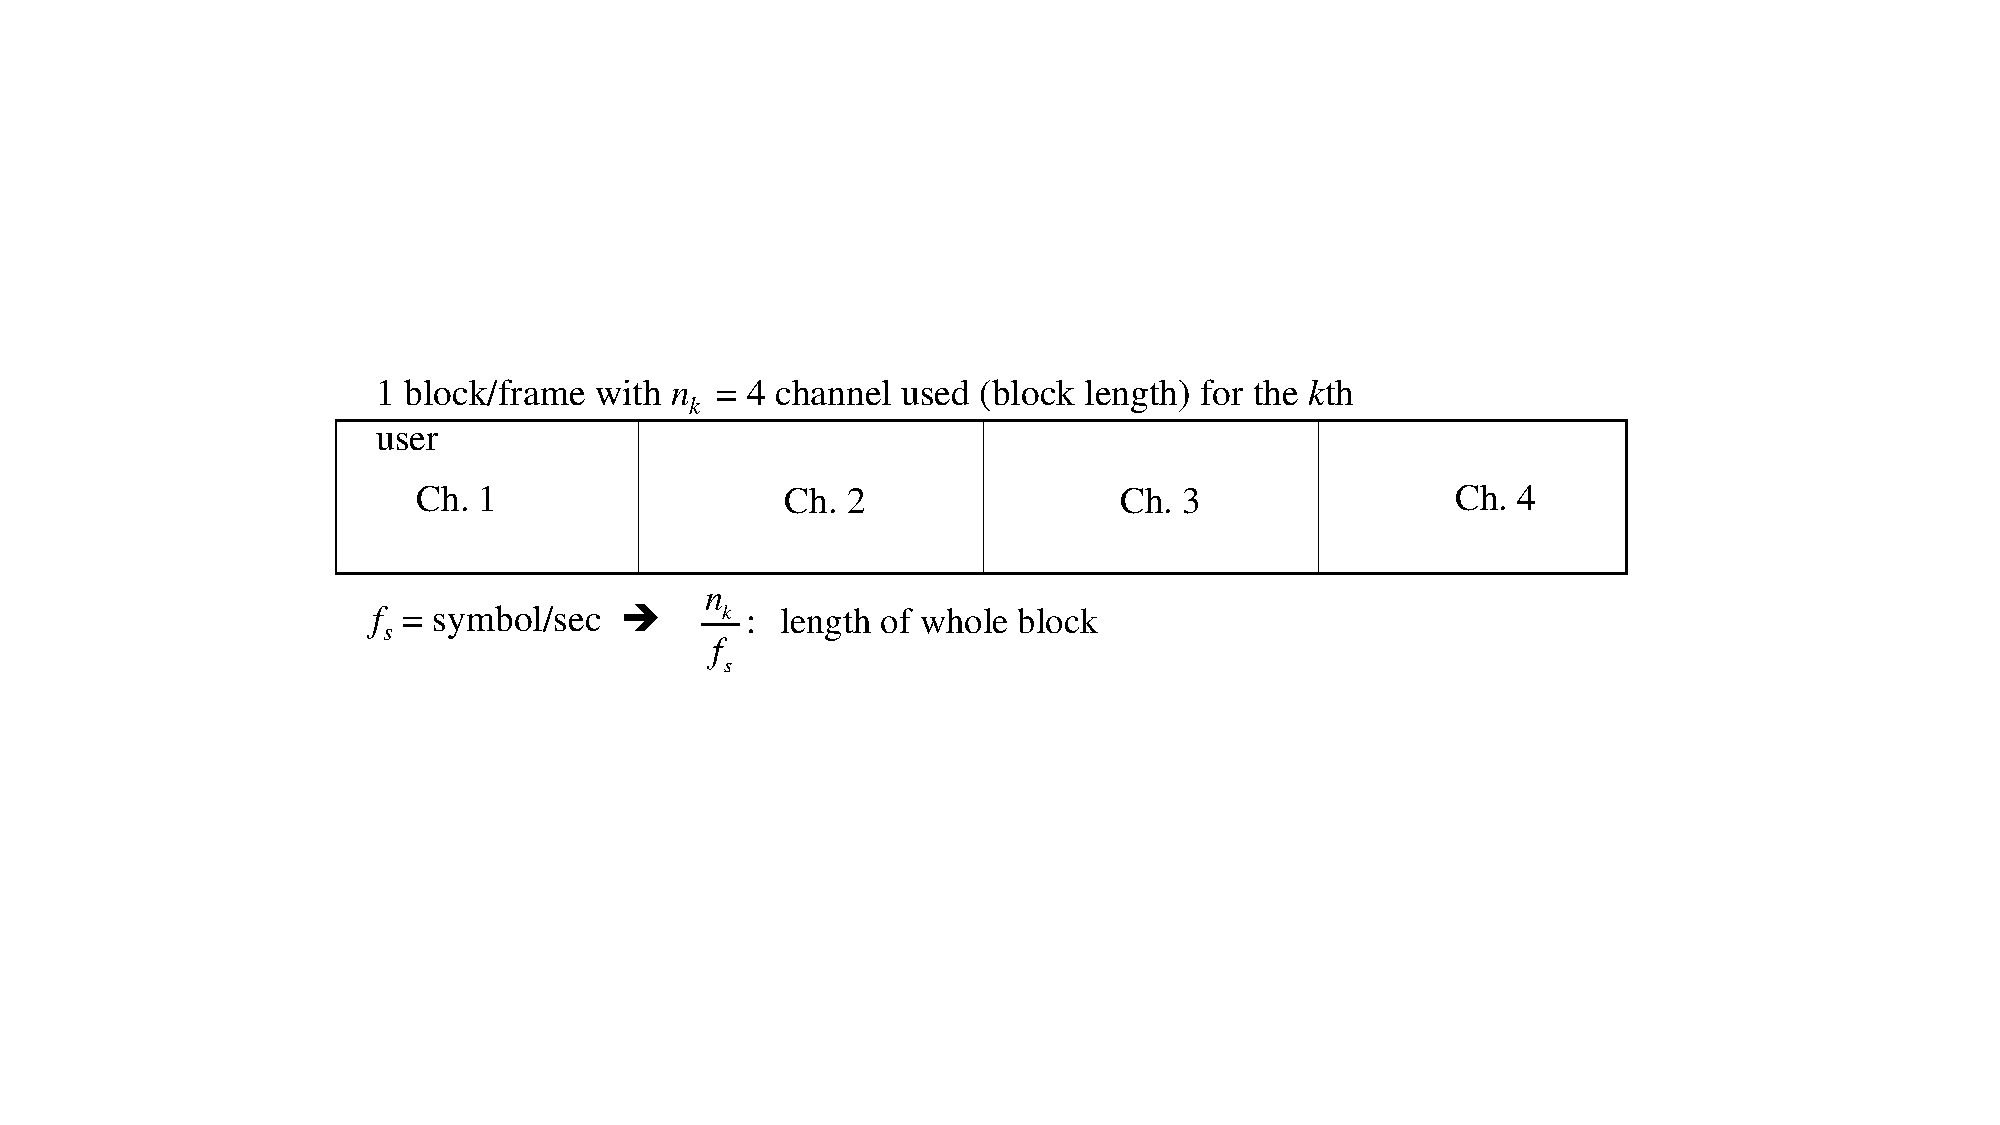
\includegraphics[width = 0.9\columnwidth]{figs/fig_symbol_blklength.pdf} 
	\caption{Illustration of blocklength (or channel used) in a block/frame of bits.  The figure shows that $n_k = 4$, so $\frac{n_k}{f_s}$ denotes the length of the whole block/frame in time (sec).} 
\label{fig_symbol_blklength}
\end{figure}
%******************************************************************

In reality most low latency application operate in the finite blocklength regime, where the number of transmitted symbols $n$ is limited. In this case in a Gaussian channel, the received signal with blocklength $n$ can be written as
\begin{equation*}
	\Y = \sum_{k=1}^K \H_K \F_k  \S_k + \W
\end{equation*}
where the received signal $\Y \in \mathbb{C}^{N_R \times n}$, the transmitted signal $\S_k \in \mathbb{C}^{d_k \times n}$, the Gaussian channel matrix $\H_k \in \mathbb{C}^{N_R \times N_k}$, the precoder matrix $\F \in \mathbb{C}^{ N_k \times d_k}$, the noise matrix $\W \in \mathbb{C}^{N_R \times n}$  and $d_k \leq N_k$.  $N_k$ denotes the number of transmitted antenna at the $k$th user.
 
However this assumes a fixed Gaussian channel, a time-varying Rayleigh fading will be considered herein. Let $T$ denote the coherence time of the channel, i.e. the number of channel uses over which the channel remains constant.  Then the blocklength (total channel uses) of a codeword can be written as
\textcolor{red}{THIS EQUATION STILL DOESN'T MAKE SENSE TO ME.  If $T$ is the channel used/coherent interval, then it should always be 1 as 1 channel used occupies 1 coherent interval}
\begin{equation*}
	n = L \times T
\end{equation*}
where $T$ is the number of channel uses over which the channel remains constant and $L$ is the number of coherent channels within one blocklength.

By considering the coherent intervals, the received signal can be written as \\
\textcolor{blue}{From now on, don't use ``l'', because that will be confused as ``1'' (one).  Use $\ell$ instead}
\begin{equation*}
	\Y = \sum_{k=1}^K \sum_{\ell = 1}^L \H_{k, } \F_{k, \ell}  \S_{k, \ell} + \W \ \in \complex^{L \times N_r \times T}
\end{equation*}
where $\Y \in \complex^{L \times N_r \times T}$, $\H_k \in \complex^{L \times N_r \times N_k}$, $\F_k \in \complex^{L \times N_k \times d_k}$, $\S_k \in \complex^{L \times d_k \times T}$

\text{\sout{(i think it can also be written as 
$Y \in \complex^{N_r \times L \times T}$, 
$\H_k \in \complex^{N_r \times L \times N_k}$, 
$\F_k \in \complex^{N_k \times L \times d_k}$, 
$\S_k \in \complex^{d_k \times L \times T}$)}}

\subsection{Problem Formulation with Rayleigh Fading Channel}
%**************************************************************************
Let $B_k$ be number of bits sent by the $k$th user, let $n_k$ be the blocklength of user $k$, let $\F_k$ be the precoder of user-$k$.  Let blocklength of user $k$ be split in coherent intervals as 
\textcolor{red}{SAME HERE. THIS EQUATION STILL DOESN'T MAKE SENSE TO ME.  If $T_K$ is the channel used/coherent interval, then it should always be 1 as 1 channel used occupies 1 coherent interval}
\begin{equation*}
	n_k = L_k \times T_K
\end{equation*}
where $L_k$ is the number of coherent intervals within the blocklength of user $k$ (cf. Fig. \ref{fig_symbol_blklength}, this can mean  bv) and $T_k$ is the number of channel uses in one coherent interval of user $k$.

A weighted latency minimization problem can be defined as 
\begin{equation}
	\begin{split}
		\min_{\F_{k,\ell}, n_k, \epsilon_k} \;& \sum_{k \in K} w_k \frac{n_k}{f_s} \\
		\text{s.t.}\;& \frac{B_k}{n_k} \leq \max_{\F_{k, \ell}} \frac{1}{L_k} \sum_{l=1}^{L_k} R^*(T_{k}, \F_{k, \ell}), \quad \forall k \in \mcK \\ 
		& n_k \in [n_{\text{min}}, n_{\text{max}}], \quad \forall k \in \mcK \\
		& \|\F_{k,\ell}\|_F^2 \leq P_{k,\ell}, \quad \forall \ell \in [0, L_k],  \forall k \in \mcK,
	\end{split}
\label{eq_short_blocklength_latency_min_prob}
\end{equation}
where the finite blocklength rate for coherent interval $\ell$ of user $k$ is defined as, 
\begin{equation*}
R^*(T_{k} , \F_{k,\ell}) =  C_k(\F_{k,\ell}) - \sqrt{ \frac{V_k(\F_{k,\ell})}{ T_{k, \ell} } } Q^{-1}  (\epsilon_k), \quad \forall \ell \in [0,L_k] \forall k \in \mcK\\
\end{equation*}
The channel variance of the $k$th user in coherence interval $\ell$ is defined as, 
\begin{equation*}
	\begin{aligned}
		V_k(P_{k,\ell}) 
		&\;\approx\; \sum_{i=1}^{N_{k, \min}} \Bigg[
    	\frac{1}{\,N_{k, \max}-i+1\,}
    		+ \frac{1}{2 (N_{k, \max}-i+1)^2}
    		+ \dots
		\Bigg] \\[0.6em]
		&\quad + N_{k, \min} (\ln e)^2 \\[0.6em]
		&\quad + \frac{(\ln e)^2}{2} \Bigg(
		N_{k, \min} - \frac{N_{k, \min}^2}{N_k}
		+ \frac{2 \Big( \frac{N_{k, \min}}{N_k} - 1 \Big)}{\alpha_{k,\ell}} 
        \sum_{i=1}^{N_{k, \min}} \mathbb{E} \Big[ \frac{1}{\lambda_{k, \ell, i}^2} \Big]
		+ \mathcal{O}\Big( \frac{1}{\alpha_{k,\ell}^2} \Big)
		\Bigg), \\[0.6em]
	\end{aligned}
\end{equation*}
where $\alpha_{k,\ell} = \frac{P_{k,\ell}}{N_k}$ is the SNR and $P_{k,\ell}$ is the transmit power. However since we are assuming an isotrophic Raylegh fading channel it is also equal to the total transmit power thus, $P_{k,\ell} = \|\F_{k,\ell}\|_F^2 $.


\subsection{Solution in case of Rayleigh Fading Channel}
%******************************************************************
\begin{equation}
	\begin{split}
		\min_{\F_{k,\ell}, n_k, \epsilon_k} \;& \sum_{k \in K} w_k \frac{n_k}{f_s} \\
		\text{s.t.}\;& \frac{B_k}{n_k} \leq \max_{\F_{k, \ell}} \frac{1}{L_k} \sum_{\ell=1}^{L_k} 		R^*(T_{k}, \F_{k, \ell}), \quad \forall k \in \mcK \\ 
		& n_k \in [n_{\text{min}}, n_{\text{max}}], \quad \forall k \in \mcK \\
		& \|\F_{k,\ell}\|_F^2 \leq P_{k,\ell}, \quad \forall \ell \in [0, L_k],  \forall k \in \mcK.
	\end{split}
\label{eq_short_blocklength_latency_min_prob}
\end{equation}
(\ref{eq_short_blocklength_latency_min_prob}) can be solved by first fixing $\F_{k,\ell}$ and finding $n_k$ via exhaustive search between $[n_{min}, n_{max}]$.  This is followed by fixing $n_k$ to the value that was found in the previous step and maximizing $R^*(T_k, \F_{k,\ell})$ to reduce the latency by increasing the upper bound in the 1st constraint of (\ref{eq_short_blocklength_latency_min_prob}). 

To convert  $R^*(T_k, \F_{k,\ell})$ into a concave function, the square root in $\sqrt{\frac{V(\F_{k,\ell})}{T_k}} Q^{-1}{(\epsilon_k)}$ is removed, followed by variable substitution by solving $\Q_{k,\ell} \triangleq \F_{k,\ell}\F_{k,\ell}^H$ instead of $\F_{k,\ell}$.  This makes $R^*(T_k, \Q_{k,\ell})$ a concave function. Then $R^*(T_k, \Q_{k,\ell})$ is maximized as 
\begin{equation}
	\begin{split}
		\max_{\F_{k,\ell} \in \mcC}  \; C_k(\F_{k,l}) - V(\F_{k,\ell}) 
&=  \max_{\F_{k,\ell} \in \mcC} \; \log \det \Big( \sigma_w^{-2} \H_{k,\ell} \F_{k,\ell} \F_{k,\ell}^H \H_{k,\ell}^H \Big)
   - \frac{V(\F_{k,\ell})}{T_k} Q^{-1}(\epsilon_k),
%&= - \min_{\Q_{k,\ell} \succeq 0} \; - \log \det \Big( \sigma_w^{-2} \H_{k,\ell} \Q_{k,\ell} \H_{k,\ell}^H \Big)
   - \frac{V(\Q_{k,\ell})}{T_k} Q^{-1}(\epsilon_k)
	\end{split}
\label{eq_max_rate}
\end{equation}
where $\displaystyle \mcC = \left\{ \F_{k,\ell} \left| \frac{B_k}{n_k} \leq \max_{\F_{k, \ell}} \frac{1}{L_k} \sum_{\ell=1}^{L_k} R^*(T_{k}, \F_{k, \ell}),   \|\F_{k,\ell}\|_F^2 \leq P_{k,\ell}, \forall \ell \in [0, L_k], \text{for } k = 1, \ldots K,   \right. \right\}$.  
The solution for both $n_k$ and $\Q_{k,\ell}$ is obtained through alternating optimization by solving (\ref{eq_short_blocklength_latency_min_prob}) and (\ref{eq_max_rate}).  Once the optimal $\Q_{k,\ell}$ is obtained, $\F_{k,\ell}$ can be found via a randomization procedure that satisfies the transmit power constraint $\|\F_{k,\ell}\|_F^2 \leq P_{k,\ell}$, $\forall \ell \in [0, L_k],  \forall k \in \mcK$ as outlined in \cite{chang2015semm}.

Since it appears to is difficult to convexify (\ref{eq_max_rate}) due to the complex nature of $V(\F_{k,\ell})$, (\ref{eq_short_blocklength_latency_min_prob}) can be solved using a neural network.  Finding $n_k$ is the same as before, i.e. using exhaustive search.  However, solving for (\ref{eq_max_rate}) will be different.  Since the problem is a constrained problem, its Lagrangian can be written as
\begin{equation*}
	\mcL (\F_{k,\ell}, \lambda_1, \lambda_2) = R^*(T_k, \F_{k,\ell}) + \lambda_1 \left( R^*(T_k, \F_{k,\ell}) - \frac{B_k}{n_k} \right) + \lambda_2 \left( P_{k,\ell} - tr\left(\F_{k,\ell} \F_{k,\ell}^H \right) \right).
\end{equation*}
(\ref{eq_max_rate}) can be solved via the primal-dual algorithm by breaking it into the following three problems
\begin{subequations}
	\begin{align}
		\F_{k,\ell}^{(i+1)} &= \argmax_{\F_{k,\ell}^{(i)}} \; \mcL (\F_{k,\ell}^{(i)}, \lambda_1^{(i)}, \lambda_2^{(i)})	\label{eq_F_soln} \\
		\lambda_1^{i+1} &= \argmin_{\lambda_1} \; \mcL (\F_{k,\ell}^{(i+1)}, \lambda_1, \lambda_2^{(i)})	\nonumber \\
		&= \left[ \lambda_1^{(i)}  - \eta_{\lambda_1}^{(i)} \left( R^*(T_k, \F_{k,\ell}^{(i+1)}) - \frac{B_k}{n_k^{(i+1)}} \right) \right]_+ 	\label{eq_lambda1_soln}	\\
		\lambda_2^{(i+1)} &= \argmin_{\lambda_2} \; \mcL (\F_{k,\ell}^{(i+1)}, \lambda_1^{(i+1)}, \lambda_2) \nonumber \\
		&=  \left[  \lambda_2^{(i)} - \eta_{\lambda_2}^{(i)} \left( P_{k,\ell} - tr\left(\F_{k,\ell}^{i+1} \F_{k,\ell}^{(i+1) \; H} \right) \right) \right]_+.
			\label{eq_lambda2_soln}
	\end{align}
	\label{eq_soln}
\end{subequations}
According to the complementary slackness condition, 
\begin{align*}
	\lambda_1 \left( R^*(T_k, \F_{k,\ell}) - \frac{B_k}{n_k} \right) &= 0 \\
	\lambda_2 \left( P_{k,\ell} - tr\left(\F_{k,\ell} \F_{k,\ell}^H \right) \right) &= 0, 
\end{align*}
which implies that either $\lambda_1 = 0$ or $R^*(T_k, \F_{k,\ell}) - \frac{B_k}{n_k} = 0$ and $\lambda_2 = 0$ or $P_{k,\ell} - tr\left(\F_{k,\ell} \F_{k,\ell}^H \right) = 0$ when the primal-dual algorithm converges.  The iteration should be terminated using the above complementary slackness conditions, as well as the other relevant KKT conditions.

(\ref{eq_F_soln}) can be solved by parameterizing the solution using a neural network with parameters $\btheta$ so that it can be found using gradient ascent
\begin{equation}
	\btheta_{k, \ell}^{(i+1)} = \btheta_{k, \ell}^{(i)} + \eta_{\btheta_{k,\ell}}^{(i)} \nabla_{\btheta_{k,\ell}^{(i)}}  \mcL (\btheta_{k,\ell}^{(i)}, \lambda_1^{(i)}, \lambda_2^{(i)}),
\label{eq_F_soln_NN}
\end{equation}
here the input to the model is the channel, the output is the precoder $\F_{k,\ell}^{(i+1)}$.  That is,  $\F_{k,\ell}^{(i)} = f\left( \h^{(i)}; \btheta_{k,\ell}^{(i)} \right)$, with $f(\cdot)$ denoting the output of the neural network parameterized by $\btheta_{k,\ell}^{(i)}$, with input $\h^{(i)}$ (the channel at the $i$th iteration).  The step sizes $\eta_{\btheta_{k,\ell}}^{(i)}$, $\eta_{\lambda_1}^{(i)}$, and $\eta_{\lambda_2}^{(i)}$ may be obtained using backtracking line search, exponential decaying sequence, or something else that decays as the iteration index $i$ increases.  Reference \cite{shi2021} and reference therein for more information about what choice of neural network you should use.

Hence, the algorithm first finds $\F_{k,\ell}^{(i+1)}$ by solving (\ref{eq_F_soln_NN}) by fixing $\lambda_1$ and $\lambda_2$ to be $\lambda_1^{(i)}$ and $\lambda_2^{(i)}$, respectively.  After obtaining $\F_{k,\ell}^{(i+1)}$, then $\lambda_1^{(i+1)}$ will be obtained using (\ref{eq_lambda1_soln}).  Finally, $\lambda_2^{(i+1)}$ will be obtained using (\ref{eq_lambda2_soln}).  Since it is $\displaystyle \frac{1}{L_k} \sum_{\ell=1}^{L_k} 		R^*(T_{k}, \F_{k, \ell})$ that needs to be maximized, variables need to be solved for all $\ell = 1, \ldots, L_k$ and $k = 1, \ldots K$.  



\subsection{Reformulating in AWGN to simplify channel dispersion}

Since precoder $\F$ was not included in Rayleigh Fading channel dispersion equation $V_{iid}(P)$ we will consider an AWGN channel for simplicity.

\begin{equation*}
	\y = \sum_{k=1}^K \F_k \s_k + \w \in \complex^{N_R},
\end{equation*}
where 
$\F_k \in \complex^{N_k \times d_k}$ denotes the precoding matrix for the $k$th user, $d_k$ denotes the number of spatial streams user $k$ is sending to the AP (and $d_k \leq N_k$), $\s_k \in \complex^{d_k}$ denotes the transmitted signal for the $k$th user, $\w \in \complex^{N_R}$  denotes the AWGN, with $N_k$ denoting the number of antennas at the $k$th user and $N_R$ denotes the number of antennas at the AP.  It is assumed that $E \left[ \s_k \s_k^H \right] = \I_{N_k}$.


The optimization problem then becomes, 

\begin{equation*}
	\begin{split}
		\min_{\F_{k,\ell}, n_k, \epsilon_k} \;& \sum_{k \in K} w_k \frac{n_k}{f_s} \\
		\text{s.t.}\;& \frac{B_k}{n_k} \leq \max_{\F_{k, \ell}} \frac{1}{L_k} \sum_{\ell=1}^{L_k} 		R^*(T_{k}, \F_{k, \ell}), \quad \forall k \in \mcK \\ 
		& n_k \in [n_{\text{min}}, n_{\text{max}}], \quad \forall k \in \mcK \\
		& \|\F_{k,\ell}\|_F^2 \leq P_{k,\ell}, \quad \forall \ell \in [0, L_k],  \forall k \in \mcK.
	\end{split}
	%\label{eq_short_blocklength_latency_min_prob}
\end{equation*}

where $R^*(T_k, \F_{k,\ell})$ is,

\begin{equation*}
	R^*(T_{k} , \F_{k,\ell}) =  C_{k,l}(\F_{k,\ell}) - \sqrt{ \frac{V_k(\F_{k,\ell})}{ T_{k, \ell} } } Q^{-1}  (\epsilon_k), \quad \forall \ell \in [0,L_k] \forall k \in \mcK\\
\end{equation*}

The Capacity and Channel Dispersion equation can be for AWGN MIMO can be derived from \cite{yuri2010} which presents the equations with SNR $\rho$.
\begin{equation*}
	\begin{aligned}
		\mathbf{A}_{k,\ell}(\F_{k,\ell}) &= \sigma^{-2} \mathbf{H}_{k,\ell} \F_{k,\ell} \F_{k,\ell}^H \mathbf{H}_{k,\ell}^H, \\[2mm]
		C_{k,\ell}(\F_{k,\ell}) &= \log_2 \det \Big( \mathbf{I} + \mathbf{A}_{k,\ell}(\F_{k,\ell}) \Big), \\[1mm]
		V_{k,\ell}(\F_{k,\ell}) &= \sum_i \frac{\lambda_i \left(\lambda_i + 2 \right)}{\left(\lambda_i + 1 \right)^2} (\log_2 e)^2 \\[1mm]
		&= \text{tr} \Big[ \mathbf{A}_{k,\ell} (\mathbf{A}_{k,\ell}+2 \mathbf{I}) (\mathbf{A}_{k,\ell} + \mathbf{I})^{-2} \Big] (\log_2 e)^2,
	\end{aligned}
\end{equation*}


To solve this optimization problem the earlier method of solving for the Lagrangian can be used, where the precoder $\F_{k,\ell}$ can be paramaterized by the neural network weights $\theta_{k,\ell}$ and gradient ascent be performed on the Lagrangian to obtain optimal precoder given the slack constraints.

\subsection{Different formulations of $R^*$ and solution}

\textbf{1. Per-Block Rate}

Each coherence block can be treated as an independent transmission. The achievable rate can be optimized per block:

\begin{equation*}
	R^*_\ell(n_{k,\ell}, \F_{k,\ell}, \H_{k,\ell}) \approx C(\F_{k,\ell}, \H_{k,\ell}) - \sqrt{\frac{V(\F_{k,\ell}, \H_{k,\ell})}{n_{k,\ell}} } \, Q^{-1}(\epsilon_k)
\end{equation*}

where $n_\ell$ is the blocklength of block $\ell$ and $\epsilon_\ell$ is the target error probability for that block. This method allows per-block latency and optimization.

\textbf{Updated Optimization Problem} 

\begin{equation*}
	\begin{split}
		\min_{\F_{k,\ell}, n_{k}, \epsilon_k} \;& \sum_{k \in K} w_k \frac{n_k}{f_s} \\
		\text{s.t.}\;& \frac{B_{k,\ell}}{n_{k,\ell}} \leq \max_{\F_{k, \ell}} R^*_\ell(n_{k,\ell}, \F_{k, \ell},  \H_\ell), \quad \forall k \in \mcK, \; \ell = 1, \ldots L_k \\ 
		& n_{k,l} \in [n_{\text{min}}, n_{\text{max}}], \quad \forall k \in \mcK, \; \ell = 1, \ldots, L_k \\
		& \|\F_{k,\ell}\|_F^2 \leq P_{k,\ell}, \quad \forall k \in \mcK, \; \ell = 1, \ldots, L_k.
	\end{split}
	%\label{eq_short_blocklength_latency_min_prob}
\end{equation*}


\textbf{Updating $B_{k, \ell}$ post optimization of $n_{k,\ell}$}

Once $n_{k, \ell}$ is minimized through the alternating optimization process.

If 
\begin{equation*}
	\frac{B_{k,\ell}}{n_{k,\ell}} > R^*_\ell(n_{k,\ell}, \F_{k, \ell})
\end{equation*}

Update and reduce $B_{k, \ell}$ to $B_{k, \ell} =  \lfloor n_{k, \ell} \times R^*_\ell(n_{k,\ell}, \F_{k, \ell}) \rfloor$

\textbf{Asynchronality Optimization}

Once blocklength optimization proccess is over, we would obtain a list of all possible $n_k$ values for user-$k$ in the interval $[n_{min}, n_{max}]$.

To solve the asynchronality we can search through the possible $n_k$ values  for user-$k$  received from the previous alternating-optimization process to find the correct $n_k$ values for each user $k$ to minimize the following objectives,


1. Weighted Average Latency 

We can use the weighted average latency, where the weights are decided by $w_{k,\ell} = \frac{1}{CNR_{k,\ell}}$ ($\frac{1}{SNR_{k,\ell}}$ in the case of AWGN).

\begin{equation*}
	\min_{\F_{k,\ell}, n_{k,\ell}} \sum_{k \in K} w_{k,\ell} \frac{n_{k,\ell}}{f_s}
\end{equation*}

\textcolor{red}{However this might just end up reducing the overall latency of the system instead of reducing the latency as there is no tradeoff(of resources) that occurs between the users to justify the use of weights.}


2. Min-Max problem


To create a more fair asynchronous optimization we use max-min optimization.

\begin{equation*}
	\min_{ \F_{k,\ell}, n_{k,\ell}} \max_{k,\ell} \sum_{\stackrel {k \in K} {\ell =1}}^{L_k} w_{k,\ell} \frac{n_{k,\ell}}{f_s}
\end{equation*}

This would ensure that the latency of the system is the same as the slowest user rendering the asynchronality to be equal to $0$.

\textbf{2. Average Rate over Coherence Blocks}

In the standard block-fading FBL model, a codeword spans multiple coherence blocks, each with independent channel realizations. The achievable rate is approximated using the expectation of capacity and dispersion over coherent blocks:

Assume there are $L$ coherent blocks, and each block has $n_l$ symbols.
\begin{equation*}
		R^*_k(n_\ell, \F_\ell, \H_\ell) = \frac{1}{n} \sum_{\ell=1}^{L_k} n_\ell C(\F_\ell, \H_\ell) - 
	\sqrt{\frac{\frac{1}{n} \displaystyle \sum_{\ell=1}^{L_k} n_\ell V(n_\ell, \F_\ell, \H_\ell)}{n}} \, Q^{-1}(\epsilon)
\end{equation*}

where $n = \sum_{\ell} n_\ell$ (total blocklength), $C(h_\ell)$ is the Shannon capacity of block $\ell$, $V(h_\ell)$ is the channel dispersion, and $\epsilon$ is the target codeword error probability.

I think this allows joint decoding while the other method doesnt.

\newpage
\subsection{Simulation of Independant Sub-block Transmission}
%*************************************************************************************
\textbf{Experiment Setup}

We consider a block-fading channel where the channel is constant over a coherence block and changes independently across different coherence blocks.

\begin{table}[H]
\centering
\caption{Table of Variables and Definitions}
\begin{tabular}{|c|l|}
\hline
\textbf{Variable} & \textbf{Definition} \\ \hline
$K$ & Number of Users \\ \hline
$L_k$ & Maximum number of subblocks (coherence blocks) for user $k$ \\ \hline
$\ell$ & Sub-block index \\ \hline
$T$ & Coherence blocklength (symbols per sub-block) \\ \hline
$N_r$ & Number of Receive Antennas \\ \hline
$N_t$ & Number of Transmit Antennas \\ \hline
$f_s$ & Symbol rate \\ \hline
$n_{k,\ell}$ & Blocklength for user $k$ at sub-block $\ell$ \\ \hline
$\epsilon_k$ & Target error probability for user $k$ \\ \hline

$\H_{k,\ell} \in \mathbb{C}^{N_r \times N_t}$ & Channel matrix \\ \hline
$\F_{k,\ell} \in \mathbb{C}^{N_t \times d_k}$ & Precoder matrix \\ \hline
$\X_{k,\ell} \in \mathbb{C}^{d_k \times n_\ell}$ & Transmitted signal \\ \hline

$B_{k, \ell}$ & Number of bits transmitted for user $k$ in sub-block $\ell$ \\ \hline
$R^*_{k,\ell}(\H_{k,\ell}, \F_{k,\ell}, n_{k,\ell})$ & Finite-blocklength rate for user $k$ in sub-block $\ell$ \\ \hline
$C_{k,\ell}(\H_{k,\ell}, \F_{k,\ell}, n_{k,\ell})$ & Shannon capacity of channel $H_{k,\ell}$ \\ \hline
$V_{k,\ell}(\H_{k,\ell}, \F_{k,\ell}, n_{k,\ell})$ & Channel dispersion of channel $H_{k,\ell}$ \\ \hline
$P_{k,\ell}$ & Transmit power constraint for user $k$ in subblock $\ell$ \\ \hline
$M_{k,\ell}$ & Modulation order for user $k$ in subblock $\ell$ \\ \hline
$\gamma_{k,\ell}$ & Signal-to-interference-plus-noise Ratio (SINR) for user $k$ in subblock $\ell$ \\ \hline
\end{tabular}
\label{tab:variables_sim}
\end{table}

\textbf{Aim}

The experiment aims to reduce the number of symbols transmitted in each sub-block
to minimize the latency of the system. This is done by optimizing
\begin{equation*}
	\begin{split}
		\min_{\F_{k,\ell}, n_{k,\ell}} \;& \sum_{\stackrel {k \in K} {\ell =1}}^{L_k} w_{k,\ell} \frac{n_{k,\ell}}{f_s} \\
		\text{s.t.}\;& \frac{B_{k,\ell}}{n_{k,\ell}} \leq \max_{\F_{k, \ell}} R^*_\ell(n_{k,\ell}, \F_{k, \ell},  \H_{k,\ell}), \quad \forall k \in \mcK, \; \ell = 1, \ldots, L_k \\ 
		& n_{k,\ell} \in [n_{\text{min}}, n_{\text{max}}], \quad \forall k \in \mcK, \; \ell = 1, \ldots L_k \\
		& \|\F_{k,\ell}\|_F^2 \leq P_{k,\ell}, \quad \forall k \in \mcK, \; \ell = 1, \ldots, L_k. 
	\end{split}
	%\label{eq_short_blocklength_latency_min_prob}
\end{equation*}


(The optimization problem has been rewritten from previous formulations to optimize per sub-block by considering each sub-block as an independent transmission)

The Capacity and Channel Dispersion equation for AWGN MIMO can be derived from \cite{yuri2010} which presents the equations as

\begin{equation}
\begin{aligned}
\mathbf{A}_{k,\ell}(\H_{k,\ell},\F_{k,\ell})
&=
\sigma^{-2}
\mathbf{H}_{k,\ell}
\F_{k,\ell}
\F_{k,\ell}^H
\mathbf{H}_{k,\ell}^H, \\[2mm]
C_{k,\ell}(\H_{k,\ell}, \F_{k,\ell})
&=
\log_2 \det \big(
\mathbf{I}
+
\mathbf{A}_{k,\ell}(\H_{k,\ell},\F_{k,\ell})
\big), \\[2mm]
V_{k,\ell}(\H_{k,\ell}, \F_{k,\ell})
&=
(\log_2 e)^2
\sum_i
\frac{\lambda_i (\lambda_i + 2)}{(\lambda_i + 1)^2},
\end{aligned}
\label{eq:capacity_dispersion}
\end{equation}

where $\lambda_i$ are the eigenvalues of $\mathbf{A}_{k,\ell}(\F_{k,\ell})$.

\begin{equation*}
	R^*_{k,\ell}(n_{k,\ell}, \F_{k,\ell}, \H_{k,\ell}) \approx C(\F_{k,\ell}, \H_{k,\ell}) - \sqrt{\frac{V(\F_{k,\ell}, \H_{k,\ell})}{n_{k,\ell}}} \, Q^{-1}(\epsilon_{k})
\end{equation*}
\textbf{Training Algorithm}

\noindent\textbf{SubBlocklength-Precoder Optimization for Training }

\begin{algorithmic}[1]
\Ensure
Feasible solutions
$\{(n_{k,\ell}^*, \F_{k,\ell}^*, R_{k,\ell}^*)\}$

\For{$k = 1$ \textbf{to} $K$} \Comment{Loop over users}

    \State Normalize channel:
    \textcolor{red}{Define a vectorized version of $\H_k$ using $\H_{k,\ell}$, use $\bmu_{\H_k}$ and $\sigma_{\H_k}$ instead} \\
    $\H_k \gets (\H_k - \mathrm{mean}(\H_k)) / \sqrt{\mathrm{var}(\H_k)}$

    \For{$\ell = 1$ \textbf{to} $L_k$} \Comment{Loop over sub-blocks}
	
		
        \State
        \textcolor{red}{Need to define $^{(0)}$ notation, $\Delta n_{k,\ell}$, $\F_{\text{init},k,\ell}$ } \\
        $\mathcal{S}_{k,\ell}
        \gets
        \textsc{OptimizeSubBlocklength-Precoder}
        (f_\theta,
        \F_{\mathrm{init}, k, \ell},
        n_{\max},
        n_{\min},
        \Delta n_{k,\ell},
        \lambda_\text{rate}^{(0)},
        \lambda_\text{power}^{(0)})$

        \State Select feasible tuple
        $(n_{k,\ell}^*, \F_{k,\ell}^*, R_{k,\ell}^*)
        = \mathcal{S}_{k,\ell}[-1]$

    \EndFor
\EndFor

\State \Return all feasible solutions
\end{algorithmic}


\newpage


\noindent\textbf{Algorithm 1: \textsc{OptimizeSubBlocklength-Precoder}}

\begin{algorithmic}[1]

\Ensure
Feasible tuples
$\{(n_\ell^*, \F_\ell^*, R_{\mathrm{FBL}}^*,
\lambda_{rate}^*, \lambda_{power}^*)\}$

\State Initialize PrecoderNet $f_\theta$ and Adam optimizer with learning rate $\eta_{\text{net}}$
\State $\lambda_{rate} \gets \lambda_{rate}^{(0)}$
\State $\lambda_{power} \gets \lambda_{power}^{(0)}$
\State $Results \gets \emptyset$

\For{$n_\ell = n_{\ell,\max}$ \textbf{to} $n_{\ell,\min}$ \textbf{step} $-\Delta n_\ell$}

\If{$n_\ell = n_{\ell,\max}$}
\Comment{(It is observed that the program takes a larger number of epochs to find the initial precoder)}
        \State $epochs \gets 2000$ 
    \Else
        \State $epochs \gets epochs_{\text{per-}n_\ell}$
    \EndIf

    \Comment{Optimize precoder for current sub-blocklength}
    \State
    $(\F^*,
    \lambda'_{rate},
    \lambda'_{power},
    R_{\mathrm{FBL}},
    c_{rate},
    c_{power},
    \mathcal{L})
    \gets
    \textsc{OptimizePrecoder}(f_\theta,
    \F_{\mathrm{init}},
    n_\ell,
    epochs,
    \lambda_{rate},
    \lambda_{power})$

    \State $\lambda_{rate} \gets \lambda'_{rate}$
    \State $\lambda_{power} \gets \lambda'_{power}$

    \If{$c_{rate} \le 0$ \textbf{and} $c_{power} \le 0$}

	\Comment{Rate and Precoder constrains are satisfied for the given sub-blocklength}
        \State
        $Results \gets Results \cup
        \{(n_\ell, \F^*, R_{\mathrm{FBL}},
        \lambda_{rate}, \lambda_{power})\}$
    \EndIf

\EndFor
\State \Return $Results$
\end{algorithmic}

\newpage

\noindent\textbf{\textsc{Algorithm 2: OptimizePrecoder}}

\begin{algorithmic}[1]

\Require
Precoder network $f_\theta$, initial precoder $\F$, number of epochs $E$, Lagrange multipliers $\lambda_{rate}, \lambda_{power}$,
learning rates $(\eta_{\text{net}}, \eta_{rate}, \eta_{power})$

\Ensure
Optimized precoder $\F^*$, updated multipliers
$(\lambda_{rate}, \lambda_{power})$, achievable rate $R_{\mathrm{FBL}}$,
constraint violations $(c_{rate}, c_{power})$

\State $Losses \gets \emptyset$

\For{$e = 1$ \textbf{to} $E$}

    \State $\F_{out} \gets f_\theta(\mathbf{H}_{kl})$

    \State Zero optimizer gradients
    \State
    $(\mathcal{L},
    R_{\mathrm{FBL}},
    P_F,
    c_{rate},
    c_{power})
    \gets
    \textsc{LagrangianLoss}(\mathbf{F_{out}}, \lambda_{rate}, \lambda_{power})$

	\Comment{Early Stopping: If rate and power constrains are satisfied for the given blocklength and optimization runs for min epochs, break the loop}
    \If{$c_{rate} \le 0$ \textbf{and} $c_{power} \le 0$ \textbf{and} $e \ge 10$}
        \State \textbf{break}
    \EndIf

    \State
    $(\lambda_{rate}, \lambda_{power})
    \gets
    \textsc{UpdateLambdas}(\lambda_{rate}, \lambda_{power},
    c_{rate}, c_{power},
    \eta_{rate}, \eta_{power})$

    \State Backpropagate $\mathcal{L}$
    \State Optimizer step
    \State Append $\mathcal{L}$ to $Losses$

\EndFor

\State $\F^* \gets f_\theta(\mathbf{H}_{kl})$
\State Project $\F^*$ to valid precoder form 

\State \Return
$\F^*$, optimizer,
$\lambda_{rate}$, $\lambda_{power}$,
$R_{\mathrm{FBL}}$, $P_F$,
$c_{rate}$, $c_{power}$, $Losses$

\end{algorithmic}

\newpage
\noindent\textbf{Algorithm 3: \textsc{LagrangianLoss}}

\begin{algorithmic}[1]

\Require
Precoder $\mathbf{F_{k,\ell}}$, dual variables $(\lambda_{rate}, \lambda_{power})$, \\
System parameters $(\mathbf{H}_{k\ell}, n_{k,\ell}, \sigma^2, \epsilon_k, B_{k,l}, P_k)$

\Ensure
Lagrangian loss $\mathcal{L}$, rate $R_{\mathrm{FBL}}$, power $\|\mathbf{F_{k,\ell}}\|_F^2$, \\
Constraint violations $(c_{rate}, c_{power})$

\State $\mathbf{A}_{k,\ell} \gets \sigma^{-2} \mathbf{H}_{k\ell} \mathbf{F_{k,\ell}} \mathbf{F_{k,\ell}}^H \mathbf{H}_{k\ell}^H$

\Statex \Comment{Compute finite-blocklength capacity}
\State $C_{k,\ell} \gets \log_2 \det(\mathbf{I} + \mathbf{A}_{k,\ell})$

\Statex \Comment{Compute channel dispersion}
\State Compute eigenvalues $\{\lambda_i\}$ of $\mathbf{A_{k,\ell}}$
\State $V_{k,\ell} \gets \sum_i \frac{\lambda_i(\lambda_i + 2)}{(\lambda_i + 1)^2} (\log_2 e)^2$

\Statex \Comment{Finite-blocklength achievable rate}
\State $R_{\mathrm{FBL}} \gets C - \sqrt{\frac{V}{n_{k,\ell}}} \, Q^{-1}(\epsilon)$

\Statex \Comment{Evaluate constraints}
\State $F_{power} \gets \|\mathbf{F_{k,\ell}}\|_F^2$
\State $c_{rate} \gets \frac{B_{k,\ell}}{n_{k,\ell}} - R_{\mathrm{FBL}}$
\State $c_{power} \gets F_{power} - P_{k}$

\Statex \Comment{Soft constraint handling (penalty only if violated)}
\Statex \Comment{LeakyReLU is used as it was observed that the algorithm does not acheive maximum rate or precoder power and plays safe to satisfy the constraints. Using LeakyReLU incentivizes a higher rate and power while giving a larger penalty to breaking them. }

\State $c_{rate} \gets \mathrm{LeakyReLU}(c_{rate})$
\State $c_{power} \gets \mathrm{LeakyReLU}(c_{power})$

\Statex \Comment{Primal Dual Lagrangian objective}
\State $\mathcal{L} \gets -R_{\mathrm{FBL}}
+ \lambda_{rate} \cdot c_{rate}
+ \lambda_{power} \cdot c_{power}$

\State \Return $(\mathcal{L}, R_{\mathrm{FBL}}, F_{power}, c_{rate}, c_{power})$

\end{algorithmic}

\newpage
\noindent\textbf{Algorithm 4: \textsc{UpdateLambda} (Primal--Dual Update)}

\begin{algorithmic}[1]

\Require
Current dual variables $(\lambda_{rate}, \lambda_{power})$, \\
Constraint violations $c_{rate}$ (rate), $c_{power}$ (power), \\
Dual step sizes $(\eta_{rate}, \eta_{power})$

\Ensure
Updated dual variables $(\lambda_{rate}, \lambda_{power})$

\Statex \Comment{This procedure performs a updation step in the primal--dual optimization }


\Statex \Comment{Update Lagrange multipliers}
\State $\lambda_{rate} \gets \lambda_{rate} + \eta_{rate} \cdot c_{rate}$
\State $\lambda_{power} \gets \lambda_{power} + \eta_{power} \cdot c_{power}$

\State $\lambda_{rate} \gets \max(0, \lambda_{rate})$
\State $\lambda_{power} \gets \max(0, \lambda_{power})$

\State \Return $(\lambda_{rate}, \lambda_{power})$

\end{algorithmic}

\newpage 

\textbf{Precoder Architecture}

\noindent\textbf{UplinkMLP PrecoderNet Architecture}

\begin{itemize}
    \item \textbf{Parameters:}
        \begin{itemize}
            \item $N_r$: Number of receive antennas
            \item $N_t$: Number of transmit antennas
            \item $d_k$: Number of data streams per user
            \item Input dimension: $in\_dim = 2 \cdot N_r \cdot N_t$ (concatenated real and imaginary parts)
            \item Output dimension: $out\_dim = 2 \cdot N_t \cdot d_k$
            \item Hidden dimension: $hidden = 4 \cdot (4 \cdot out\_dim)$
        \end{itemize}

    \item \textbf{Input:} Flattened channel matrix $H_{k\ell} \in \mathbb{C}^{N_r \times N_t}$
        \begin{itemize}
            \item Real and imaginary parts concatenated: $\text{vec}([H_{k\ell}]_\text{real}, [H_{k\ell}]_\text{imag}) \in \mathbb{R}^{in\_dim}$
        \end{itemize}

    \item \textbf{Fully Connected Layers:}
        \begin{enumerate}
            \item Linear($in\_dim \rightarrow hidden$), ReLU
            \item Linear($hidden \rightarrow hidden/2$), ReLU
            \item Linear($hidden/2 \rightarrow hidden/4$), ReLU
            \item Linear($hidden/4 \rightarrow out\_dim$)
        \end{enumerate}
        
    \item \textbf{Output:} Precoder vector $F_\text{out} \in \mathbb{R}^{out\_dim}$, representing real and imaginary parts of the precoder for the sub-block.
\end{itemize}



\begin{tabular}{|c|c|c|}
\hline
Layer & Input $\rightarrow$ Output & Activation \\
\hline
Input & $in\_dim = 2 N_r N_t$ & - \\
Linear 1 & $in\_dim \rightarrow hidden = 4 \cdot (4 \cdot out\_dim)$ & ReLU \\
Linear 2 & $hidden \rightarrow hidden/2$ & ReLU \\
Linear 3 & $hidden/2 \rightarrow hidden/4$ & ReLU \\
Linear 4 & $hidden/4 \rightarrow out\_dim = 2 N_t d_k$ & - \\
\hline
Output & $out\_dim = 2 N_t d_k$ & - \\
\hline
\end{tabular}

\newpage


\textbf{Testing Algorithm}

\noindent\textbf{Sub-Blocklength per User Testing}

\begin{algorithmic}[1]

\Require
Number of users $K$, simulation parameters
$(n_{\ell,\max}, n_{\ell,\min}, \Delta n_\ell)$,
Trained precoders $\{\F_{k,\ell}\}$, channel statistics 
$(\mu_k, \sigma_k^2)$ for all $k$ from training

\Ensure
Rate histories $\{\mathcal{R}_k\}_{k=1}^K$,
blocklength histories $\{\mathcal{N}_{k}\}_{k=1}^K$,
Bits per Symbol histories $\{\mathcal{B}_{k}\}_{k=1}^K$

\For{$k = 1$ \textbf{to} $K$}

    \State $\mathbf{H}_k \gets (\mathbf{H}_k - \mu_k)/\sqrt{\sigma_k^2}$

    \State Initialize:
    $\mathcal{R}_k \gets \emptyset$,
    $\mathcal{N}_{k} \gets \emptyset$,
    $\mathcal{B}_{k} \gets \emptyset$

    \For{$\ell = 1$ \textbf{to} $L_k$}

        \State Initialize histories:
        $\mathcal{R}_{k,\ell} \gets \emptyset$,
        $\mathcal{N}_{k,\ell} \gets \emptyset$,
        $\mathcal{B}_{k, \ell} \gets \emptyset$

        \State Load trained precoder $\F_{k,\ell}$

        \For{$n_\ell = n_{\ell,\max}$ \textbf{to} $n_{\ell,\min}$ \textbf{step} $-\Delta n_\ell$}

            \State Set blocklength $n_\ell$ for user $k$, block $\ell$

            \State Compute achievable rate $R_{\mathrm{FBL}}^{k,\ell}$
            \State Compute required rate per symbol $B_k / n_\ell$

            \If{$\dfrac{B_k}{n_\ell} > R_{\mathrm{FBL}}^{k,\ell}$}
                \Statex \Comment{Constraint violated: minimum feasible blocklength reached}
                \State Restore blocklength to $n_\ell + \Delta n_\ell$
                \State \textbf{break}
            \EndIf

            \State Append $R_{\mathrm{FBL}}^{k,\ell}$ to $\mathcal{R}_{k,\ell}$
            \State Append $n_\ell$ to $\mathcal{N}_{k,\ell}$
            \State Append $B_k/n_\ell$ to $\mathcal{B}_{k, \ell}$

        \EndFor

        \State Append $\mathcal{R}_{k,\ell}$ to $\mathcal{R}_k$
        \State Append $\mathcal{N}_{k,\ell}$ to $\mathcal{N}_{k}$
        \State Append $\mathcal{B}_{k, \ell}$ to $\mathcal{B}_{k}$

    \EndFor

\EndFor

\State \Return $\left(\{\mathcal{R}_k\}, \{\mathcal{B}_{k}\}, \{\mathcal{N}_{k}\}\right)$

\end{algorithmic}




\newpage
\textbf{Problems with this approach}

The problems with this approach stem from how we initialize the simulation.

An example initial paramters for 2 identical users used in the current simulation is as follows:

\begin{tabular}{|l|c|c|}
\hline
\textbf{Parameter} & \textbf{User 1} & \textbf{User 2} \\
\hline
Number of users $K$ & \multicolumn{2}{c|}{2} \\
\hline
Receive antennas $N_r$ & 16 & 16 \\
Transmit antennas $N_t$ & 4 & 4 \\
\hline
Number of sub-blocks $L_k$ & 5 & 5 \\
Bits per sub-block $B_{k,l}$ & 500 & 500 \\
\hline
Symbols per sub-block(coherent block) $T_{k}$ & 250 & 250 \\
Initial sub-block length $n_{k,\ell}$ & 250 & 250 \\
\hline
SNR (dB) & 5.0 & 5,0 \\
Transmit power $P_t$ & 20.0 & 20.0 \\
\hline
Symbol frequency $f_s$ (Hz) & 15{,}000 & 15{,}000 \\
Target error probability $\epsilon$ & $10^{-10}$ & $10^{-10}$ \\
\hline
Training seed & \multicolumn{2}{c|}{0} \\
Testing seed & \multicolumn{2}{c|}{1} \\
\hline 
\end{tabular} \\


The initial parameters assume the number of sub-blocks $L$, this is a problem as the number of sub-blocks is derived from the equation $L_k = N_k/T$, where $T$ (coherence time) is the only channel constant, where $\displaystyle N_k \triangleq \sum_{\ell = 1}^{L_k} n_{k,\ell}$

Thus it is not right to set the initial value of $L$ as it is a derived quantity.

As the current algorithm reduces the sub-blocklength $n_{k,\ell}$,  this could create a scenario post-optimization where due to reducing $n_l$ and having constant $T$, sub-block $l$ has less symbols and could also contain the symbols of the next sub-block.

For example assume,

$T = 200,$
$n_1 = 200,$
$n_2 = 200,$
$L = 2,$

post optimization we optimize $n_1$ and $n_2$ to become,

$T=200,$
$n_1 = 100,$
$n_2 = 80$

Thus in this scenario sub-block $1$ can hold symbols of sub-block $1$ and sub-block $2$.

This is because $n_1(100) + n_2(80) < T(200)$, thus all the symbols can fit in the first coherant block.

\newpage

\textbf{Proposed Solution}

Lets remove initial values of $L_k$ and $n_{k,\ell}$ and rewrite the initial parameters to only contain total bits $B_k$ and coherence time $T_{k,\ell}$.

Thus the rewritten initial parameters are as follows:

\begin{tabular}{|l|c|c|}
\hline
\textbf{Parameter} & \textbf{User 1} & \textbf{User 2} \\
\hline
Number of users $K$ & \multicolumn{2}{c|}{2} \\
\hline
Receive antennas $N_r$ & 16 & 16 \\
Transmit antennas $N_t$ & 4 & 4 \\
\hline
Total Bits per user $B_k$ & 5000 & 5000 \\
\hline
Coherence time of user $k$ in subblock $\ell$: $T_{k,\ell}$ & 250 & 250 \\
\hline
SNR (dB) & 5.0 & 5,0 \\
Transmit power $P_{k,\ell}$ (\textcolor{red}{Units?  Should be in dBm}) & 20.0 & 20.0 \\
\hline
Symbol frequency $f_s$ (Hz) & 15{,}000 & 15{,}000 \\
Target error probability $\epsilon_k$ & $10^{-10}$ & $10^{-10}$ \\
\hline
Training seed & \multicolumn{2}{c|}{0} \\
Testing seed & \multicolumn{2}{c|}{1} \\
\hline 
\end{tabular} \\

We will try to solve the problem of changing $L_k$ to a derived quantity by assuming initial value of $L_k = 1$ and $n_{k,\ell} = T_{k,\ell}$.

This means initially all of user bits $B_k$ is encoded into $T_{k,\ell}$ symbols ($n_{k,\ell} = T_{\k,\ell}$) within a single sub-block (coherent block) ($L_k = 1$).
Thus initially the simulation has a high bit/symbol ratio of $B_k/n_{k,\ell} = B_k/T_{\k,\ell}$ which corresponds to a higher modulation order of $M_{k, \ell} = 2^{B_k/T_{k,\ell}}$, where $\displaystyle B_k \triangleq \sum_{\ell=1}^{L_k} B_{k,\ell}$ is the total number of bits transmitted from user $k$. 

However this might not satisfy the rate and power constraints, then we try to optimize $L_k$ and $B_{k,\ell}$ by reducing the sub-blocklength($n_{k,\ell}$) to satisfy the constraints.

--\> If the sub-blocklength $n_{k,\ell} = T_{\k,\ell}$ does not satisfy the rate and power constraints, then we reduce $B_{k,\ell}$ in the range $[B_k, 1]$ until the constraints are satisfied.
    Then $B_{k}$ is then updated to $B_{k} = B_{k} - B_{k,\ell}$

--\> If remaining $B_{k} >0 $, then we increase $L_k = L_k+1$ and repeat the process on the next sub-block until all bits are encoded into sub-blocks ie: remaining $B_k = 0$.



Thus instead of fixing the number of sub-blocks $L_k$ and sub-blocklengths $n_{k,\ell}$ \emph{a priori}, we derive them dynamically from the total remaining bits and coherence time. Starting from a $n_{k,\ell} = T_{k,\ell}$ sub-blocklength transmission, the sub-blocklength $n_{k,\ell}$ is progressively decreased until the rate and power constraints are satisfied. If reduction is not possible, the transmitted bits are split across multiple sub-blocks.

I believe this is also optimal as having less number of sub-blocks $L_k$ with its high sub-blocklength (i.e. having sub-locklength ($n_{k,\ell} = $)  coherence interval ($T_k$)) results in lower latency in the current simulation as compared to more sub-blocks with lower sub-blocklengths.  I do not have a proof for this but i believe an intuitive explanation is the fact that having a lower $n_{k,\ell}$ results in a larger \textbf{dispersion penalty} (i.e. the channel dispersion) thus reducing the overall rate. This results in a higher total $n_{k,\ell}$ and thus higher latency when you sum the smaller $n_{k,\ell}$ across more sub-blocks. 
Thus it is better to have less sub-blocks $L_k$ with higher sub-blocklength $n_{k,\ell}$ (bounded by the coherence time $T_{k,\ell}$) than more number of sub-blocks $L_k$ with lower sub-blocklength $n_{k,\ell}$.

The refined algorithm is as follows:


\noindent\textbf{Algorithm: Dynamic SubBlocklength-Precoder Optimization for Training}
\begin{algorithmic}[1]

\Require
User payloads $\{B_k\}_{k=1}^K$, coherence blocklengths $\{T_k\}_{k=1}^K$,\\
Channels $\{\mathbf{H}_k\}_{k=1}^K$,\\
Initial dual variables $(\lambda_{rate}^{(0)}, \lambda_{power}^{(0)})$,\\
Sub-block parameters $(n_{\min}, \Delta n_\ell)$

\Ensure
Number of sub-blocks $\{L_k\}$, sub-blocklengths $\{n_{k,\ell}^*\}$, precoders $\{\F_{k,\ell}^*\}$, rates $\{R_{k,\ell}^*\}$

\For{$k = 1$ \textbf{to} $K$} \Comment{Loop over users}

    \State Normalize channel:
    $\mathbf{H}_k \gets (\mathbf{H}_k - \mathrm{mean}(\mathbf{H}_k)) / \sqrt{\mathrm{var}(\mathbf{H}_k)}$

    \State $B_k^{\mathrm{rem}} \gets B_k$
    \State $L_k \gets 1$
    \State $\ell \gets 0$
    \State $n_{\max} \gets T_k$

    \While{$B_k^{\mathrm{rem}} > 0$}
        \State
        $\mathcal{S}_{k,\ell}
        \gets
        \textsc{OptimizeSubBlocklength-Precoder}(
        f_\theta,
        \F_{\mathrm{init}},
        n_{\ell,\max},
        n_{\ell,\min},
        \Delta n_\ell,
        \lambda_{rate}^{(0)},
        \lambda_{power}^{(0)})$

        \State
        $(n_{k,\ell}^*, \F_{k,\ell}^*, R_{k,\ell}^*)
        \gets \mathcal{S}_{k,\ell}[-1]$ \Comment{Select smallest feasible blocklength}
        

        \State
        $B_{k,\ell}
        \gets
        \min\!\left(
			B_k^{\mathrm{rem}},
			\left\lfloor n_{k,\ell}^* \cdot R_{k,\ell}^* \right\rfloor
			\right)$
			\Comment{Determine transmitted bits in this sub-block}
			
        \State $B_k^{\mathrm{rem}} \gets B_k^{\mathrm{rem}} - B_{k,\ell}$
		\If{$B_k^{\mathrm{rem}} > 0$}
			\State $L_k \gets L_k + 1$
			\State $\ell \gets \ell + 1$
		\EndIf
    \EndWhile

\EndFor

\State \Return
$(\{L_k\}, \{n_{k,\ell}^*\}, \{\F_{k,\ell}^*\}, \{R_{k,\ell}^*\})$

\end{algorithmic}

\newpage


\section{Latency Minimization when number of sub-blocks($L_k$) is unknown}

Our old problem formulation considered the number of sub-blocks $L_k$ to be known and bits to be transmitted in each sub-block $B_{k,\ell}$ to be known by setting them as simulation parameters.

Inorder to remove $L_k$ as a simulation parameter , we consider a system where sub-blocks arrive sequentially and we greedily optimize the bits sent per sub-block to acheive minimum latency. 

\paragraph*{Old Problem Formulaton}

Users $k \in \{0, \dots, K-1\}$ transmit a payload of bits $B_k$ in an uplink system to a Base Station. Each user has a coherance blocklength of $T_k$ symbols and symbol rate(symbols/sec) of $fs_k$.

The problem formulation for reduction of latency can be defined as,


\begin{equation*}
\begin{aligned}
\min_{\F_{k, \ell} ,\,n_{k,\ell}} \quad
& \sum_{k \in \mathcal{K}} w_k \frac{\sum_{\ell=0}^{L_k-1} n_{k,\ell}}{fs_k} \\
\text{s.t.}\quad
& \frac{B_{k,\ell}}{n_{k,\ell}} \le
C_{k,\ell}(\F_{k, \ell} )
-\sqrt{\frac{V_{k,\ell}(\F_{k, \ell} )}{n_{k,\ell}}}\,Q^{-1}(\varepsilon_k),
\quad \forall k \in \mathcal{K},\ \forall \ell \in \{0,\dots,L_k-1\} \\
& n_{k,\ell} \in [n_{\min}, n_{\max}],
\quad \forall k \in \mathcal{K},\ \forall \ell \in \{0,\dots,L_k-1\} \\
& \|\F_{k, \ell} \|_{\F}^{2} \le P_{k,\ell},
\quad \forall k \in \mathcal{K},\ \forall \ell \in \{0,\dots,L_k-1\}.
\end{aligned}
\end{equation*}


where $\ell \in \{0,\dots,L_k-1\}$ is the sub-block, $L_k$ is the total number of sub-blocks of user $k$. $B_{k,\ell}$ is the number of bits sent by user $k$ at sub-block $\ell$, $n_{k,\ell}$ is the number of symbols sent by user $k$ at sub-block $l$.


%===============================
% Concise mathematical program
%===============================
\paragraph*{New problem formulation}
\begin{equation}
\begin{aligned}
\min_{n_{k,\ell},B_{k,\ell},\F_{k, \ell}}
&\quad \sum_{k \in \mathcal{K}}\frac{\sum_{\ell=0}^{L_k-1} n_{k,\ell}}{fs_k} \\
\text{s.t.}\quad
&\quad \frac{B_{k,\ell}}{n_{k,\ell}}
\le
C_{k,\ell}(\F_{k, \ell} )
-\sqrt{\frac{V_{k,\ell}(\F_{k, \ell} )}{n_{k,\ell}}}\,Q^{-1}(\varepsilon_k),\;\;\forall k \in \mathcal{K},\ \forall \ell \in \{0,\dots,L_k-1\} ,\\
&\quad \sum_{\ell=1}^{L_k} B_{k,\ell}=B_k, \\
&\quad 1\le n_{k,\ell}\le T_k,\;\; B_{k,\ell}\in\mathbb{Z}_{\ge 0},\;\; L_k\in\mathbb{Z}_{\ge 1},\\
&\quad \|\F_{k, \ell} \|_F^2\le P_{k,\ell},\;\;\forall k \in \mathcal{K},\ \forall \ell \in \{0,\dots,L_k-1\}  .
\end{aligned}
\end{equation}

%=========================================================
% Mathematical program of the SOLUTION ALGORITHM (abstract)
%=========================================================

\subsection{Solution Algorithm}

For each user $k$ and sub-block $\ell$, define:
\begin{align}
AO(B_{k,\ell}, T_k, \epsilon_k)
&= (n^*_{k,\ell}, \F^*_{k,\ell}) =
\arg\min_{\substack{n_{k,\ell}\in\{1,\dots,T_k\} \\ \F}}
n_{k,\ell}
\quad
\text{s.t.}\;
\frac{B_{k,\ell}}{n_{k,\ell}}
\le
C_{k,\ell}(\F_{k, \ell})
-
\sqrt{\frac{V_{k,\ell}(\F_{k, \ell})}{n_{k,\ell}}}
Q^{-1}(\varepsilon_k),
\nonumber\\
&\hspace{5.8cm}
\|\F\|_F^2 \le P_{k,\ell}.
\label{eq:oracle_N}
\\[8pt]
B^*_{k,\ell}(n_{k,\ell}, \F_{k, \ell}, \epsilon_k)
&=
\arg\max_{B_{k,\ell}\in\mathbb{Z}_{\ge0}}
B_{k,\ell}
\quad
\text{s.t.}\;
\frac{B_{k,\ell}}{n_{k,\ell}}
\le
C_{k,\ell}(\F_{k, \ell})
-
\sqrt{\frac{V_{k,\ell}(\F_{k, \ell})}{n_{k,\ell}}}
Q^{-1}(\varepsilon_k),
\nonumber\\
&\hspace{5.8cm}
\|\F_{k, \ell}\|_F^2 \le P_{k,\ell}.
\label{eq:oracle_B}
\end{align}


\begin{algorithm}[H]
\caption{Greedy Allocation of Bits for User $k$}
\textbf{Input:} Total bits $B_k$ \\
\textbf{Output:} $\{(n^*_{k,\ell},\F^*_{k,\ell},B^{\text{tx}}_{k,\ell})\}_{\ell=1}^{L_k}$
\begin{algorithmic}[1]

\State Initialize $\ell \gets 0$
\State $B{_\text{rem}}^{(\ell)}_k \gets B_k$

\While{$B{_\text{rem}}^{(\ell)}_k > 0$}

\State \textbf{Step 1: Blocklength and precoder update}

\begin{equation*}
(n^*_{k,\ell},\mathbf{F}^*_{k,\ell})
=
AO_{k,\ell}\big(B^{(\ell)}_{k,\text{rem}}, T_k, \epsilon_k \big)
\end{equation*}


\State \textbf{Step 2: Maximum transmittable bits}

\begin{equation*}
B^{\text{tx}}_{k,\ell}
=
\min
\Big\{
B{_\text{rem}}^{(\ell)}_k,
B^*_{k,\ell}(n^*_{k,\ell},\F^*_{k,\ell}, \epsilon_k)
\Big\}
\end{equation*}

\State \textbf{Step 3: Update remaining bits}

\begin{equation*}
B{_\text{rem}}^{(\ell+1)}_k = B{_\text{rem}}^{(\ell)}_k - B^{\text{tx}}_{k,\ell}
\end{equation*}

\State $\ell \gets \ell + 1$

\EndWhile

\State $L_k \gets \ell$

\end{algorithmic}
\end{algorithm}

where $B{_\text{rem}}^{(\ell)}_k$ is the remaining bits to transmit at each sub-block $l$ during the running of the algorithm,  $n^*_{k, \ell}$ is the optimal sub-blocklength of user $k$ sub-block $l$, $F^*_{k, \ell}$ is the optimal precoder, $B^{\text{tx}}_{k, \ell}$ is the number of bits transmitted at user $k$ and sub-block $l$.


\subsection{Defining $B^*_{k,\ell}(n_{k,\ell}, \F_{k, \ell}, \epsilon_k)$}

\begin{equation*}
B^*_{k,\ell}(n_{k,\ell}, \F_{k, \ell})
=
\left\lfloor
n_{k,\ell} \times
\left(
C_{k,\ell}(\F_{k, \ell})
-
\sqrt{\frac{V_{k,\ell}(\F_{k, \ell})}{n_{k,\ell}}}
\,Q^{-1}(\varepsilon_k)
\right)
\right\rfloor
\end{equation*}

\subsection {Defining  $AO(B_{k, \ell}, T_k, \epsilon_k)$ }

Alternating Optimization between $n_{k,\ell}$ and $\F_{k, \ell}$.

Given a target number of bits $B_{k,\ell}$, the pair $(n_{k,\ell},\F_{k, \ell} )$ is obtained by solving

\begin{equation}
(n_{k,\ell},\F_{k, \ell} ) =
\arg\min_{n_{k,\ell},\F_{k, \ell} } \; n_{k,\ell}
\end{equation}

subject to

\begin{equation}
\frac{B_{k,\ell}}{n_{k.\ell}}
\le
C_{k,\ell}(\F_{k, \ell} )
-
\sqrt{\frac{V_{k,\ell}(\F_{k, \ell} )}{n_{k,\ell}}}
Q^{-1}(\varepsilon_k),
\qquad
\|\F_{k, \ell} |_F^2 \le P_{k,\ell}.
\end{equation}

Since the problem is non–convex in $(n_{k, \ell},\F_{k, \ell})$ jointly, it is solved using 
\paragraph*{Alternating optimization $AO (n_{k,\ell},\F_{k, \ell})$.}
Let $i\in\{0,1,2,\dots\, I_{\max}\}$ denote the AO iteration index within sub-block $\ell$ of user $k$.
Initialize $\F_{k, \ell}^{(0)}$ and set $i=0$.
\begin{algorithm}[H]
\caption{Alternating Optimization for $AO(B_{k, \ell}, T_k, \epsilon_k)$}
\textbf{Input:} $B_{k,\ell},\,T_k,\,\varepsilon_k$ \\
\textbf{Output:} $(n^*_{k,\ell},\F^*_{k,\ell})$
\begin{algorithmic}[1]

\State Initialize $\F_{k, \ell}^{(0)}$, choose $n_{k,\ell}^{(0)}$, set $i=0$

\While{$i < I_{\max}$ and $n_{k, \ell} > 1$}

\State \textbf{Step 1: Sub-blocklength update}

\State Compute the smallest feasible blocklength
\begin{equation*}
n_{k,\ell}^{(i+1)}
=
\arg \min_{n\in\{1,\dots,T_k\}}
\left\{
n :
\frac{B_{k,\ell}}{n}
\le
C_{k,\ell}(\F_{k, \ell}^{(i)})
-
\sqrt{\frac{V_{k,\ell}(\F_{k, \ell}^{(i)})}{n}}
Q^{-1}(\varepsilon_k)
\right\}.
\end{equation*}

\If{no feasible $n$ exists}
\State $n_{k,\ell}^{(i+1)} \gets T_k$
\EndIf



\State \textbf{Step 2: Precoder update}

\begin{equation*}
\F_{k, \ell}^{(i+1)} =
\arg\min_{\F_{k, \ell}}
\;
\frac{B_{k,\ell}}{n_{k,\ell}^{(i+1)}} -
\left(
C_{k,\ell}(\F_{k, \ell})
-
\sqrt{\frac{V_{k,\ell}(\F_{k, \ell})}{n_{k,\ell}^{(i+1)}}}
Q^{-1}(\varepsilon_k)
\right)
\end{equation*}

\begin{equation*}
\text{s.t.}\quad
\|\F_{k, \ell}\|_F^2 \le P_{k,\ell}.
\end{equation*}
\State $i \gets i+1$

\EndWhile

\State $(n^*_{k,\ell},\F^*_{k,\ell}) \gets (n_{k,\ell}^{(i)},\F_{k, \ell}^{(i)})$

\end{algorithmic}
\end{algorithm}
\paragraph*{Precoder Update for fixed $n_{k,\ell}$ }

Precoder $\F(\theta_{k,\ell})$ is parameterized by a neural network $f(\theta_{k,\ell})$:
\begin{equation*}
\F(\theta_{k,\ell}) = f(\theta_{k,\ell}).
\end{equation*}

Introduce dual variables $\lambda_{1,k,\ell}\ge 0$ (FBL rate constraint) and $\lambda_{2,k,\ell}\ge 0$ (power constraint). Define the constraint residuals
\begin{equation*}
c_{1,k,\ell}(\theta_{k,\ell})
 = 
\frac{B_{k,\ell}}{n_{k,\ell}}
-\left[
\left(
C_{k,\ell}(\F(\theta_{k,\ell}))
-
\sqrt{\frac{V_{k,\ell}(\F(\theta_{k,\ell}))}{n_{k,\ell}}}\,
Q^{-1}(\varepsilon_k)
\right) \right],
\end{equation*}
\begin{equation*}
c_{2,k,\ell}(\theta_{k,\ell})
=
\|\F(\theta_{k,\ell})\|_F^2 - P_{k,\ell}.
\end{equation*}

The Loss/Lagrangian is
\begin{equation*}
\mathcal{L}_{k,\ell}(\theta_{k,\ell},\lambda_{1,k,\ell},\lambda_{2,k,\ell})
= -\left(
R^*_{k,\ell}\!\left(n_{k,\ell},\F(\theta_{k,\ell})\right)
-\lambda_{1,k,\ell}\, c_{1,k,\ell}(\theta_{k,\ell})
-\lambda_{2,k,\ell}\, c_{2,k,\ell}(\theta_{k,\ell}),
 \right) \end{equation*}
where
\begin{equation*}
R^*_{k,\ell}(n,\F_{k, \ell})
=
C_{k,\ell}(\F_{k, \ell})
-
\sqrt{\frac{V_{k,\ell}(\F_{k, \ell})}{n_{k, \ell}}}\,Q^{-1}(\varepsilon_k).
\end{equation*}

\textbf{(1) Primal update (neural parameters):}
\begin{equation*}
\theta_{k,\ell}^{(i+1)}
=
\theta_{k,\ell}^{(i)}
-
\eta_{\theta}^{(i)}
\nabla_{\theta_{k,\ell}}
\mathcal{L}_{k,\ell}\!\left(
\theta_{k,\ell}^{(i)},\lambda_{1,k,\ell}^{(i)},\lambda_{2,k,\ell}^{(i)}
\right).
\end{equation*}

\textbf{(2) Dual updates (projected):}
\begin{equation*}
\lambda_{1,k,\ell}^{(i+1)}
=
\left[
\lambda_{1,k,\ell}^{(i)}
+
\eta_{\lambda_1}^{(i)}\, g_{1,k,\ell}\!\left(\theta_{k,\ell}^{(i+1)}\right)
\right]_+,
\qquad
\lambda_{2,k,\ell}^{(i+1)}
=
\left[
\lambda_{2,k,\ell}^{(i)}
+
\eta_{\lambda_2}^{(i)}\, g_{2,k,\ell}\!\left(\theta_{k,\ell}^{(i+1)}\right)
\right]_+,
\end{equation*}
\begin{equation*}
[x]_+ := \max(x,0.1 \times x).\end{equation*}

\subsection{Results}


\subsection*{Basic Configuration}

\begin{table}[H]
\centering
\caption{Base Configuration Parameters ($K$ = number of users)}
\begin{tabular}{ll}
\toprule
\multicolumn{2}{c}{\textbf{Test Configuration}} \\
\midrule
Number of users ($K$) & 4 \\
Receive antennas  at Base Station ($N_r$) & $16$ \\
Transmit antennas per user ($Nt_{k}$) & $4$ \\
Initial bits per symbol & $[4,4,4,4]$ \\
Symbol frequency $fs_k$ (Hz) & $[15000,15000,15000,15000]$ \\
Error tolerance ($\epsilon_k$) & $[10^{-10},10^{-10},10^{-10},10^{-10}]$ \\
Seed (train / test) & $0 / 1$ \\
\midrule
\multicolumn{2}{c}{\textbf{Simulation Configuration}} \\
\midrule
Initial $\lambda_{\text{rate}}$ & 0.1 \\
Initial $\lambda_{\text{power}}$ & 0.1 \\
Epochs for precoder training per $n_l$ & 2000 \\
Learning rate (network) & 0.01 \\
Learning rate (rate constraint) & 0.01 \\
Learning rate (power constraint) & 0.01 \\
\bottomrule
\end{tabular}
\end{table}

\subsubsection*{\textbf{Experiment 0}}
Experiment 0 uses the following per-user configuration:
$T=\{10,15,20,30\}$, $\mathrm{SNR}=\{20,20,20,20\}$, $P_t=\{30,30,30,30\}$, $B=\{200,400,800,1600\}$. 
Here we simulate users with lower coherence blocklength $T$ having lower SNR and lower precoder power.

\begin{figure}[H]
    \centering
    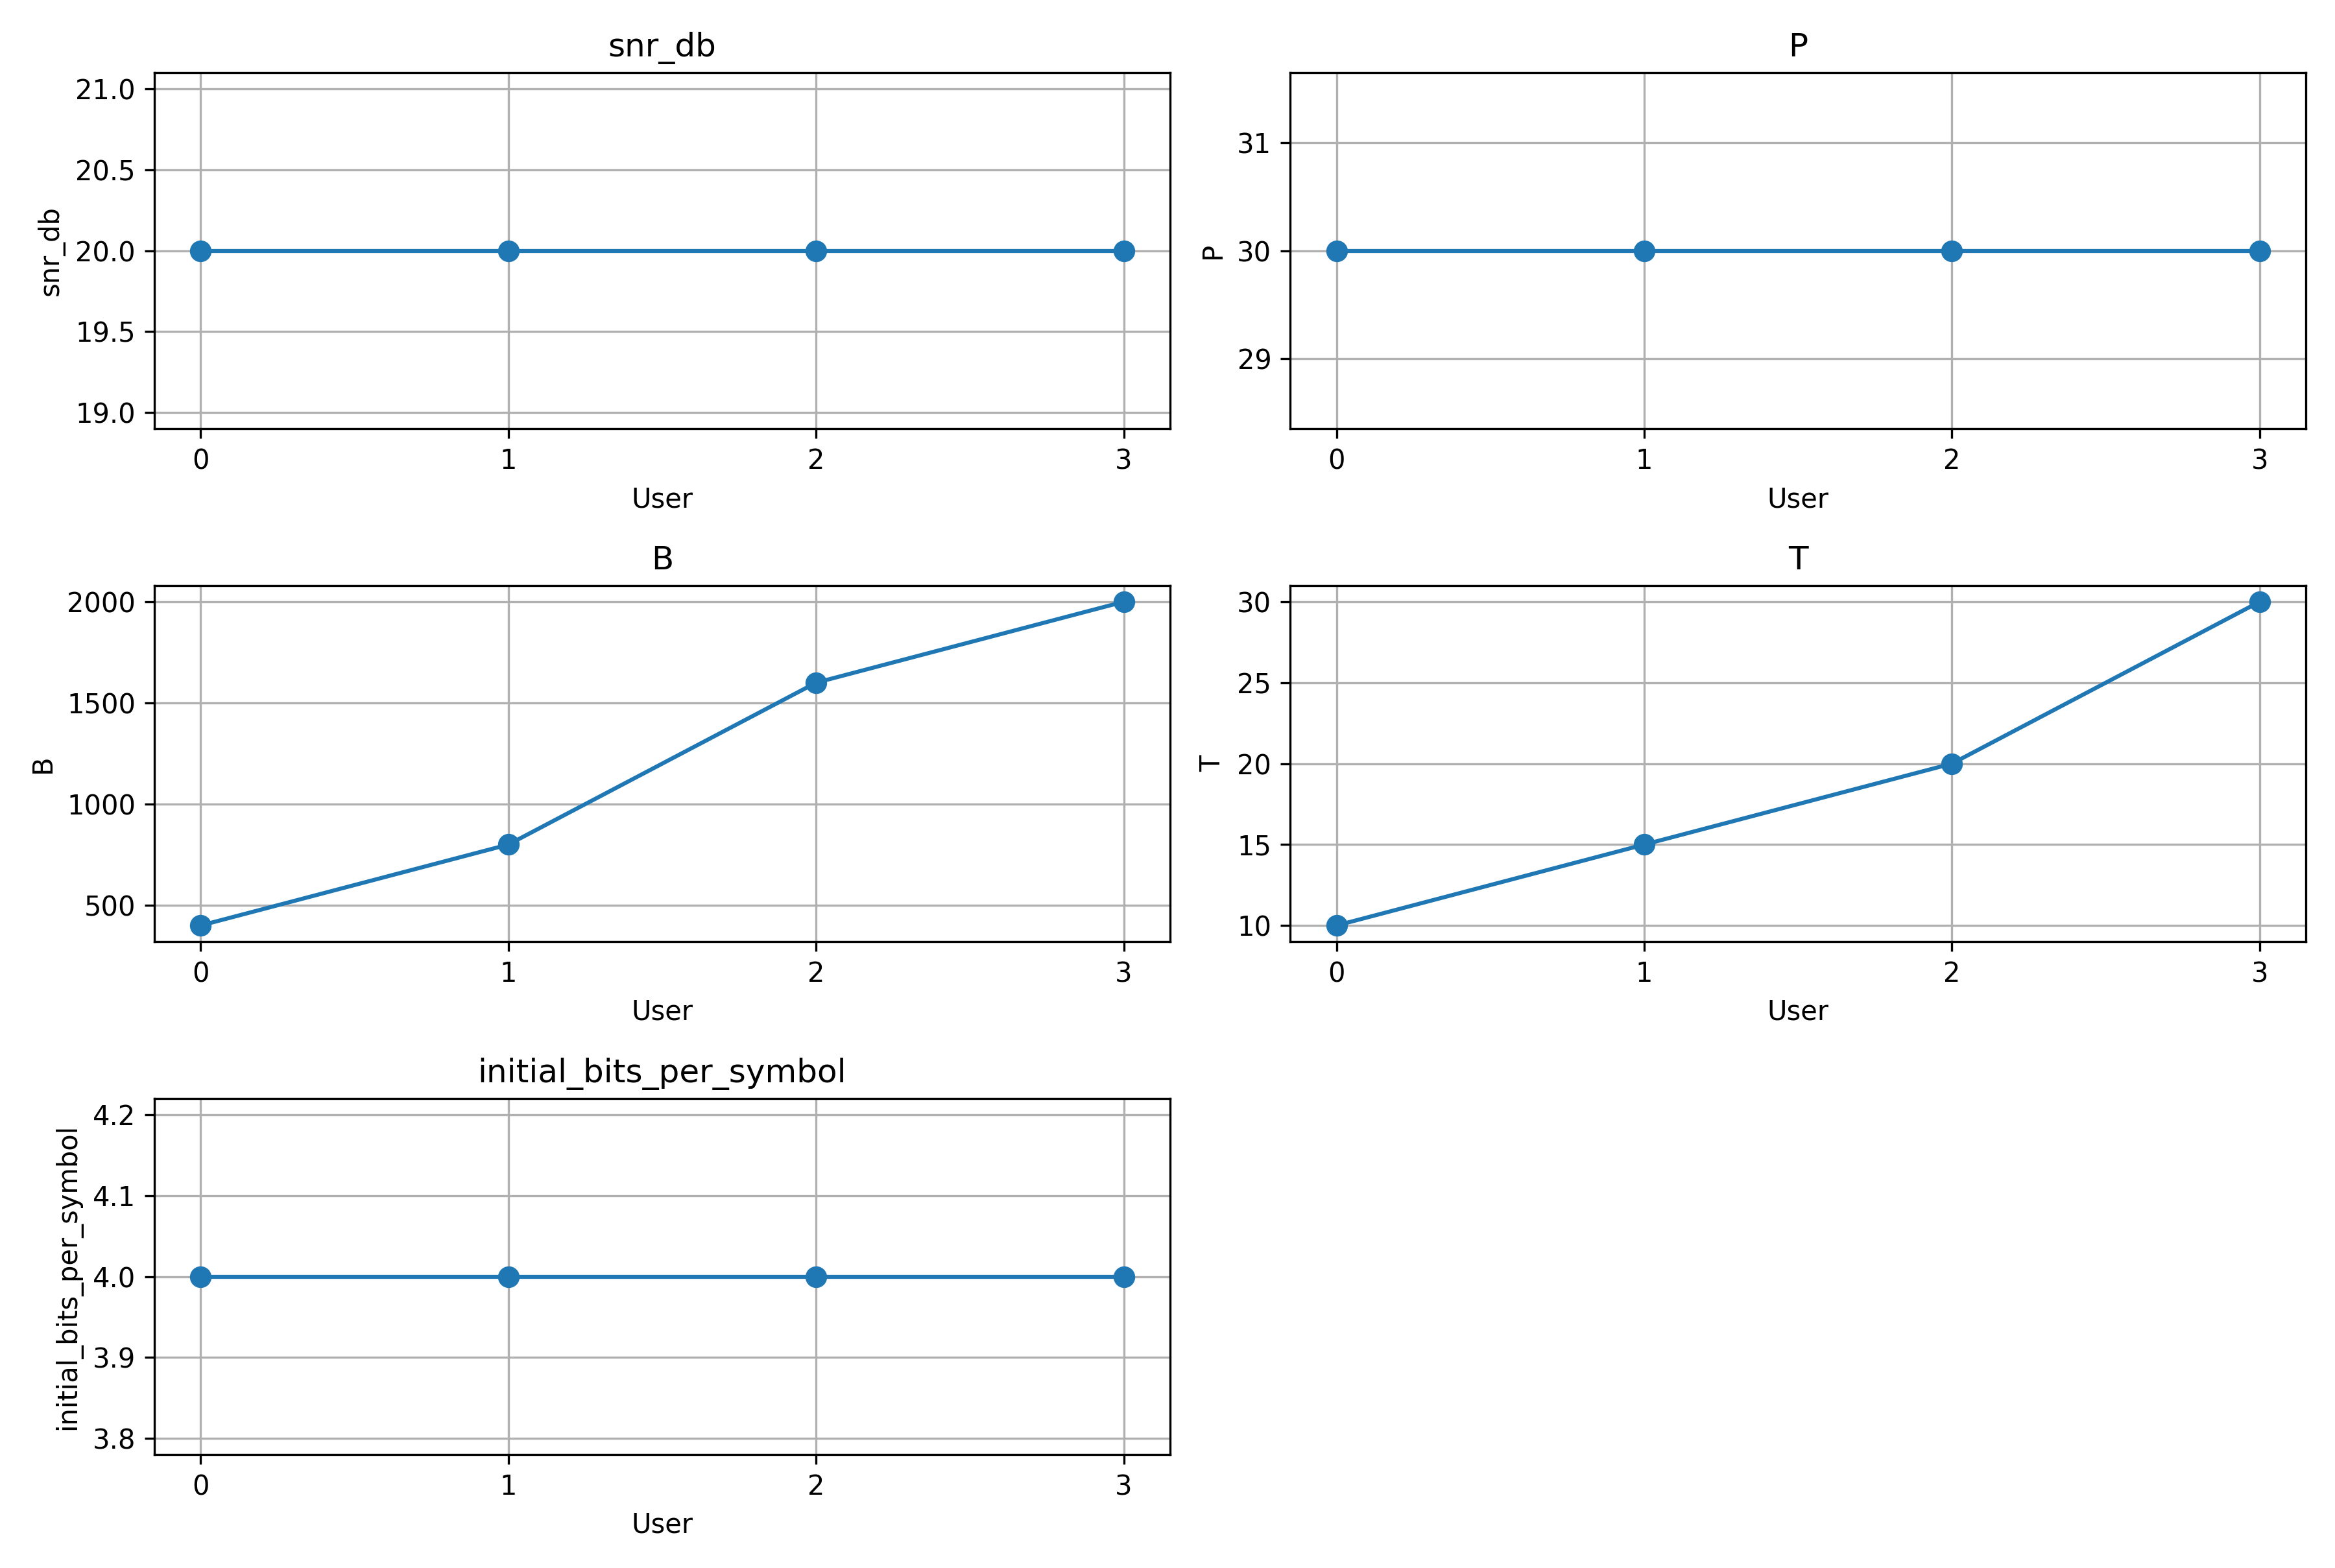
\includegraphics[width=0.9\textwidth]{figs/exp_0/exp0_cfg.png} 
    \caption{Experiment configuration parameters: SNR, Power ($P$), Bandwidth ($B$), and Time ($T$) per user.}
    \label{fig:config_overview}
\end{figure}


\begin{table*}[h]
\centering
\caption{Latency Optimization Results Per User}
\begin{tabular}{c|c|c|c|c|c|c}
\hline
User & Initial $n_k$ & Final $n_{k,\ell}$ & Initial $B_k$ & Final $B_{k,\ell}^{\text{tx}}$ & Initial $R-{\text{fsbl}}_{k, \ell}$ & Final $R_{\text{fsbl}}$ \\
\hline
0 & 50  & [7]        & 200  & [200]        & 24.5186 & [30.2743] \\
1 & 100 & [14]       & 400  & [400]        & 24.6491 & [30.0369] \\
2 & 200 & [20, 8]    & 800  & [597, 203]   & 23.1378 & [29.8853, 27.0512] \\
3 & 400 & [30, 27]   & 1600 & [851, 749]   & 24.1628 & [28.3816, 28.1232] \\
\hline
\end{tabular}

\vspace{0.5cm}

\begin{tabular}{c|c|c|c}
\hline
Metric & Initial & Final & Reduction (\%) \\
\hline
Total Latency & 0.0500 & 0.00707 & 85.87 \\
Sum Asynchronality & 0.07667 & 0.01093 & 85.74 \\
\hline
\end{tabular}
\end{table*}

% ---------------------------------------------------------
% USER 0
% ---------------------------------------------------------
\subsection*{User 0 Results}
\begin{figure}[H]
    \centering
    
\includegraphics[width=0.7\textwidth]{figs/exp_0/testing_optimization_user0_block0.png}
    \caption{Optimization performance for User 0, Block 0: Rate vs. Blocklength $n_{kl}$.}
    \label{fig:user0_results}
\end{figure}
\FloatBarrier % Forces User 0's image to stay in this section

% ---------------------------------------------------------
% USER 1 (Assuming file exists in your directory)
% ---------------------------------------------------------
\subsection*{User 1 Results}
\begin{figure}[H]
    \centering
    
\includegraphics[width=0.7\textwidth]{figs/exp_0/testing_optimization_user1_block0.png}
    \caption{Optimization performance for User 1, Block 0.}
    \label{fig:user1_results}
\end{figure}
\FloatBarrier

% ---------------------------------------------------------
% USER 2
% ---------------------------------------------------------
\subsection*{User 2 Results}
\begin{figure}[H]
    \centering
    \begin{subfigure}[b]{0.48\textwidth}
        \centering
        
\includegraphics[width=\linewidth]{figs/exp_0/testing_optimization_user2_block0.png}
        \caption{Block 0}
    \end{subfigure}
    \hfill
    \begin{subfigure}[b]{0.48\textwidth}
        \centering
        
\includegraphics[width=\linewidth]{figs/exp_0/testing_optimization_user2_block1.png}
        \caption{Block 1}
    \end{subfigure}
    \caption{User 2 optimization across multiple blocks.}
    \label{fig:user2_results}
\end{figure}
\FloatBarrier

% ---------------------------------------------------------
% USER 3
% ---------------------------------------------------------
\subsection*{User 3 Results}
\begin{figure}[H]
    \centering
    \begin{subfigure}[b]{0.48\textwidth}
        \centering
        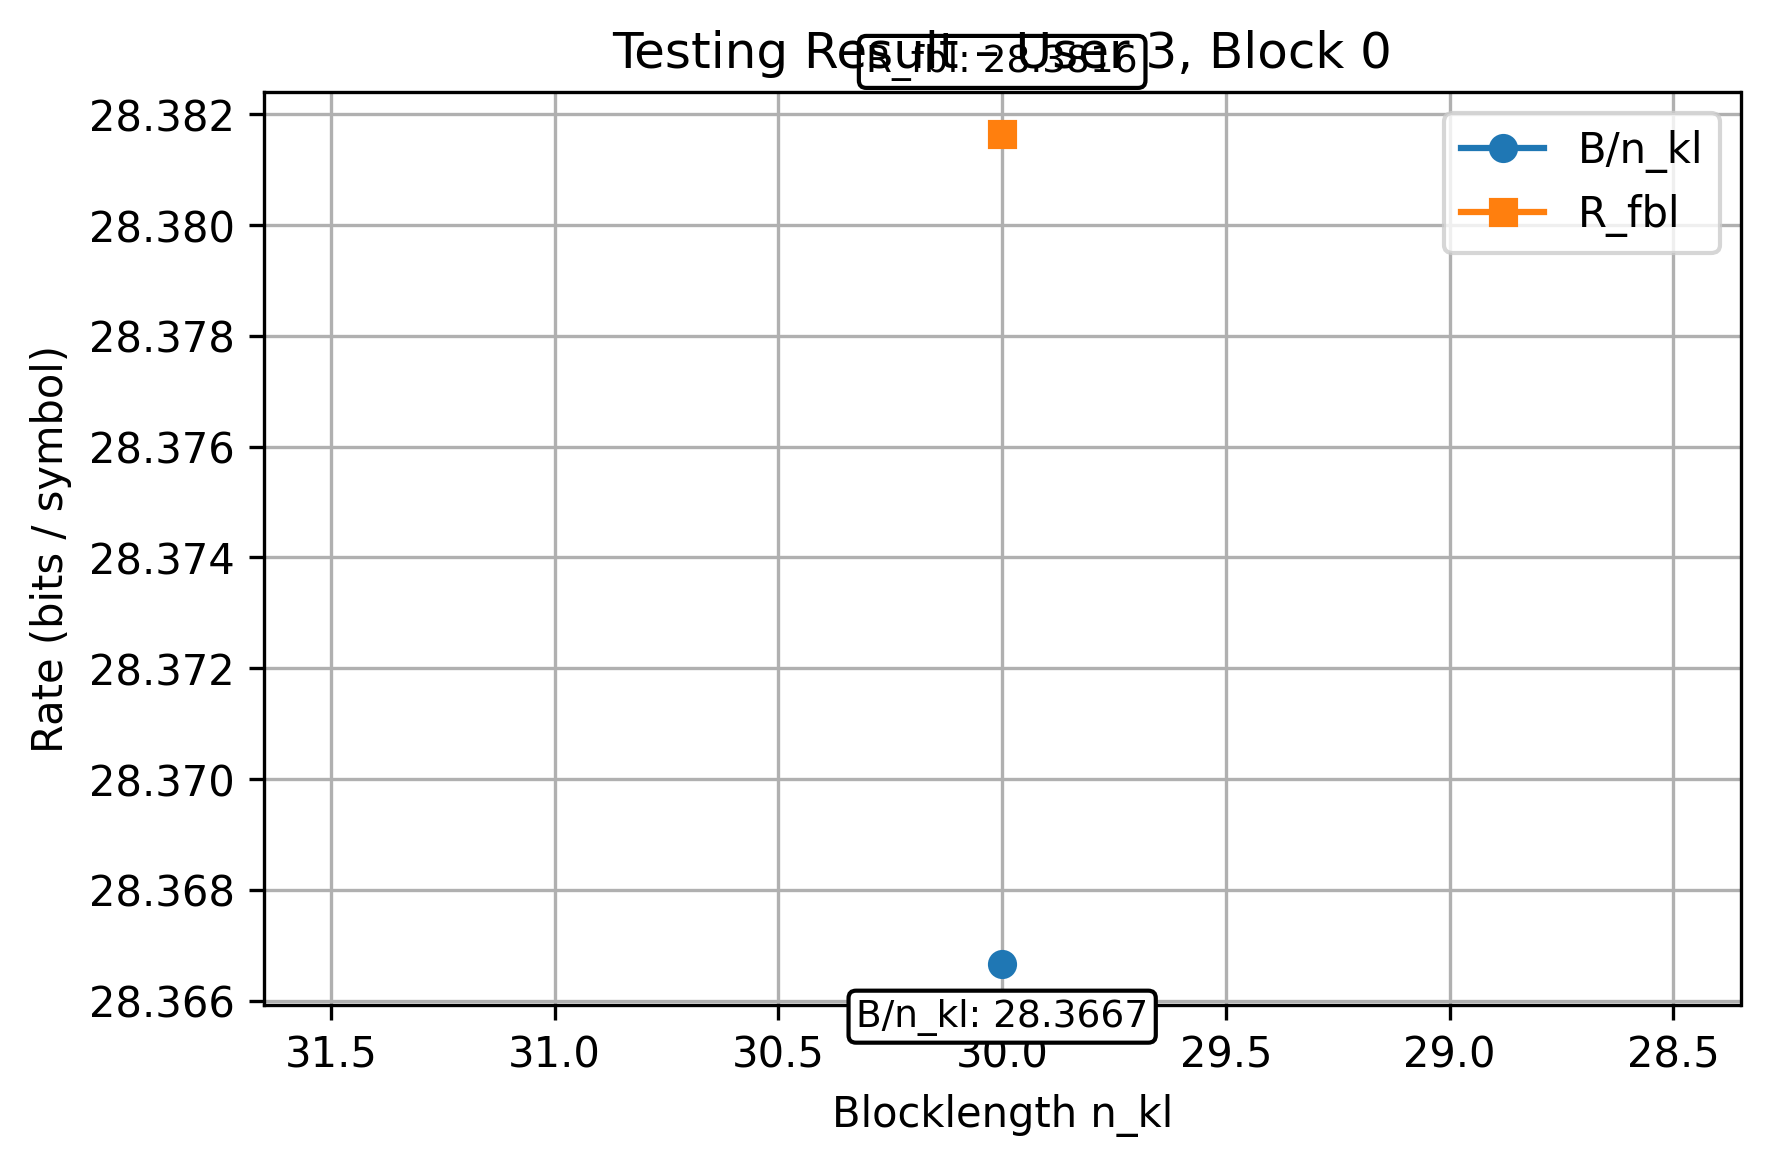
\includegraphics[width=\linewidth]{figs/exp_0/testing_optimization_user3_block0.png}
        \caption{Block 0}
    \end{subfigure}
    \hfill
    \begin{subfigure}[b]{0.48\textwidth}k
        \centering
        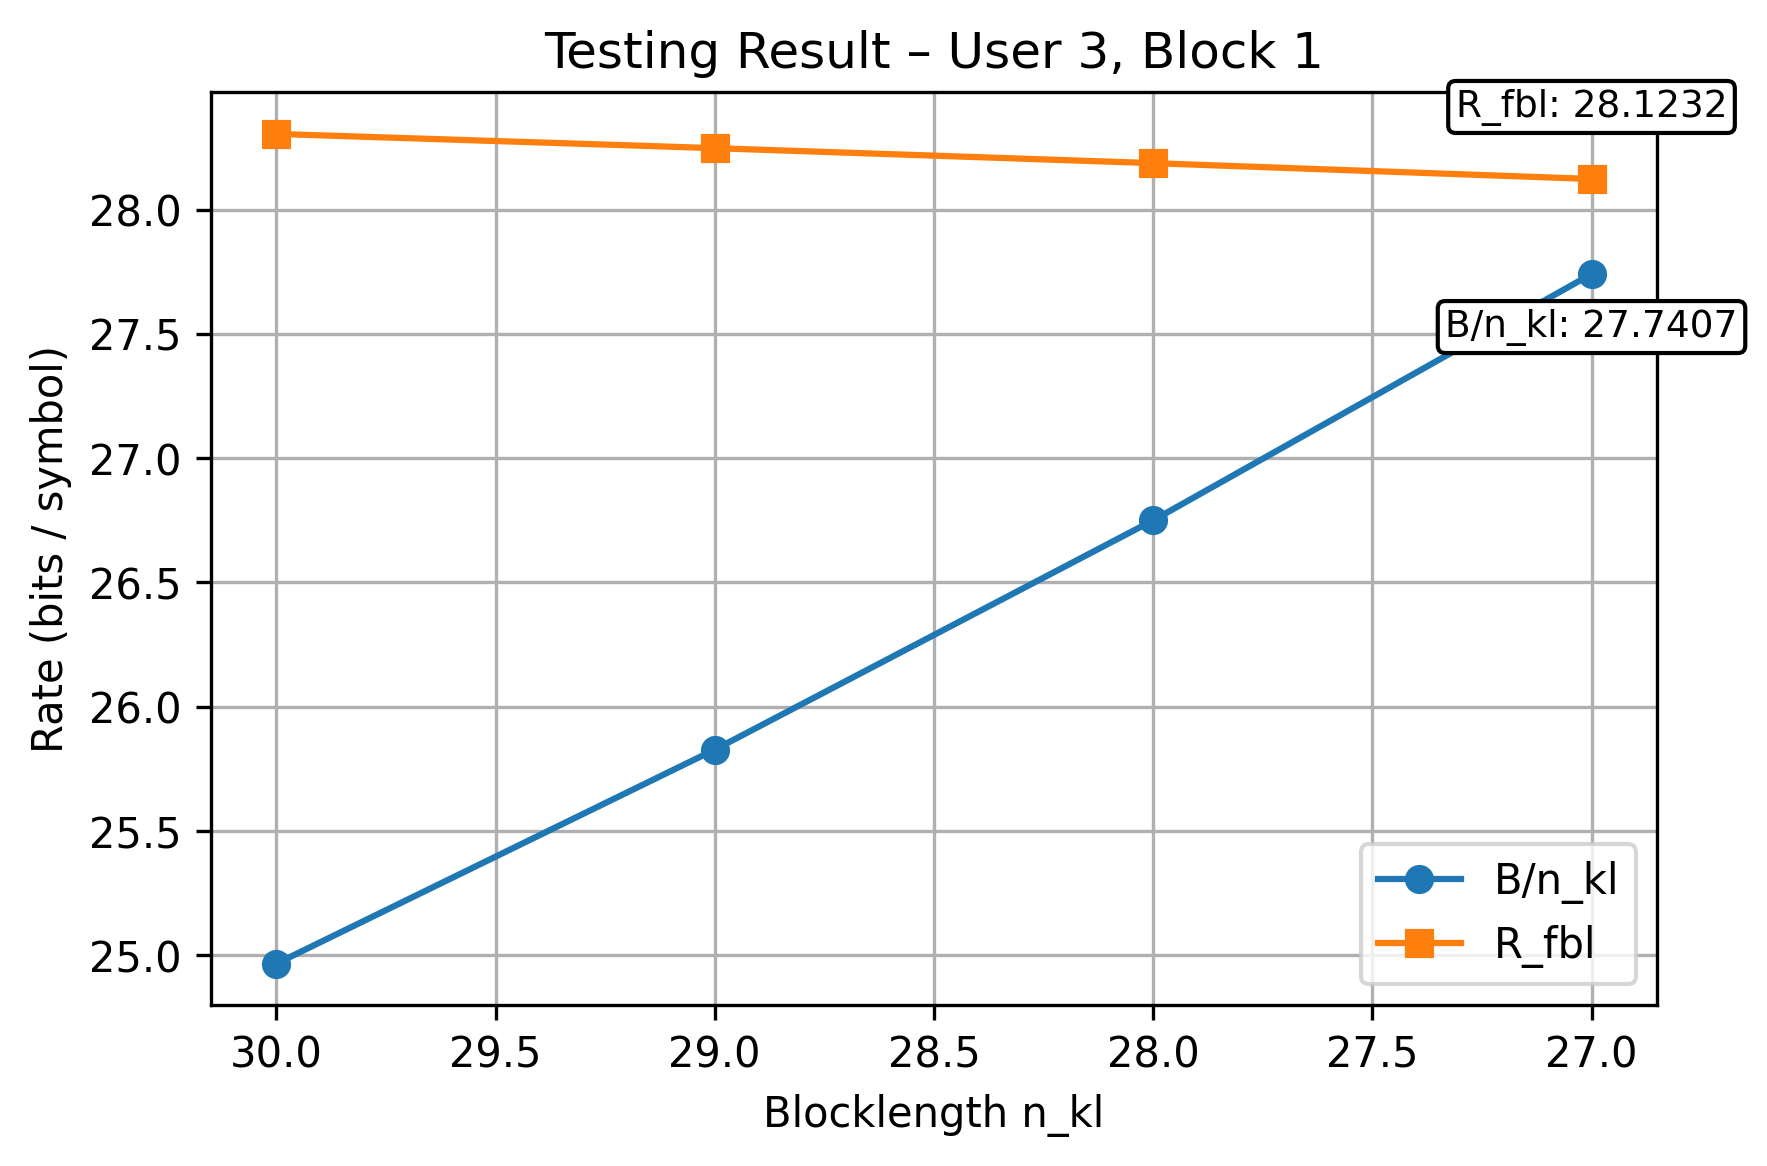
\includegraphics[width=\linewidth]{figs/exp_0/testing_optimization_user3_block1.png}
        \caption{Block 1}
    \end{subfigure}
    \caption{User 3 optimization across multiple blocks.}
    \label{fig:user3_results}
\end{figure}
\FloatBarrier

The optimization graph of initial sub-block(block 0) of user $2$ and $3$ are just points and not curves because once maximum amount of bits are fit into the sub-block it is not possible to reduce the sub-blocklength $n_{k,\ell}.$


However the final sub-block(block $1$) of users $2$ and $3$ are curves because it is possible to reduce $n_{k, \ell}$ for the remaining bits that need to be transmitted.



\begin{figure}[H]
    \centering
    % Top Row: Latency Comparison
    \begin{subfigure}[b]{0.8\textwidth}
        \centering
        
\includegraphics[width=\linewidth]{figs/exp_0/test_latency_comparison.png}
        \caption{Latency comparison ($K=4$).}
    \end{subfigure}
    \\[2ex] 
    % Bottom Row: Heatmaps
    \begin{subfigure}[b]{0.48\textwidth}
        \centering
        
\includegraphics[width=\linewidth]{figs/exp_0/test_initial_async_heatmap.png}
        \caption{Initial Asynchronality}
    \end{subfigure}
    \hfill
    \begin{subfigure}[b]{0.48\textwidth}
        \centering
        
\includegraphics[width=\linewidth]{figs/exp_0/test_final_async_heatmap.png}
        \caption{Final Asynchronality}
    \end{subfigure}
    \caption{System-wide synchronization results for Experiment 0.}
    \label{fig:latency_performance_exp0}
\end{figure}

\newpage
\subsection*{100 User Experiment}

% \subsubsection*{User Configuration}
\begin{figure}[H]
    \centering
    
\includegraphics[width=0.95\textwidth]{figs/exp_k100/user_config_reverse_summary.png}
    \caption{Configuration summary of the 100-user experiment.}
    \label{fig:exp_k100_user_config_summary}
\end{figure}

% \subsubsection{Asynchronality and Latency Statistical Results}

% Grouping the statistical summary plots together
\begin{figure}[H]
    \centering
    \begin{subfigure}[b]{0.48\textwidth}
        \centering
        
\includegraphics[width=\linewidth]{figs/exp_k100/test_latency_histogram.png}
        \caption{Latency Stats (Hist+CDF)}
    \end{subfigure}
    \hfill
    \begin{subfigure}[b]{0.48\textwidth}
        \centering
        
\includegraphics[width=\linewidth]{figs/exp_k100/test_async_distribution.png}
        \caption{Global Async Distribution}
    \end{subfigure}
    \caption{Overview of optimization performance for $K=100$.}
    \label{fig:stats_k100}
\end{figure}

\begin{minipage}{\textwidth}
    % \subsubsection{User Comparison and Heatmaps}
    \begin{figure}[H]
        \centering
        \begin{subfigure}[b]{0.95\textwidth}
            \centering
            
\includegraphics[width=\linewidth]{figs/exp_k100/test_latency_comparison.png}
            \caption{Individual Latency comparison ($K=100$).}
        \end{subfigure}
        \\[3ex] 
        \begin{subfigure}[b]{0.48\textwidth}
            \centering
            
\includegraphics[width=\linewidth]{figs/exp_k100/test_initial_async_heatmap.png}
            \caption{Initial Asynchronality}
        \end{subfigure}
        \hfill
        \begin{subfigure}[b]{0.48\textwidth}
            \centering
            
\includegraphics[width=\linewidth]{figs/exp_k100/test_final_async_heatmap.png}
            \caption{Final Asynchronality}
        \end{subfigure}
        \caption{System-wide synchronization results for 100-user scale.}
        \label{fig:latency_performance_k100}
    \end{figure}
\end{minipage}

\FloatBarrier

\begin{table}[h]
\centering
\begin{tabular}{l c}
\hline
Metric & Value \\
\hline
Total Latency Reduction (\%) & 65.83 \\
Initial Asynchronality Sum & 69.70 \\
Final Asynchronality Sum & 21.31 \\
Asynchronality Reduction (\%) & 69.43 \\
\hline
\end{tabular}
\caption{Performance comparison before and after optimization.}
\end{table}
\newpage
\begin{thebibliography}{25}
\bibitem{rimoldi1996}
B. Rimoldi and R. Urbanke, ``A rate-splitting approach to the Gaussian multiple-access channel,'' \emph{IEEE Trans. Inf. Theory},  vol. 42, no. 2, pp. 364–375, Mar. 1996.

\bibitem{yang2019}
Z. Yang, M. Chen, W. Saad, W. Xu and M. Shikh-Bahaei, ``Sum-rate maximization of uplink rate splitting multiple access (RSMA) communication,'' \emph{Proc. of the IEEE Global Communications Conference (GLOBECOM)}, Waikoloa, HI, USA, pp. 1-6, 2019.  doi: 10.1109/GLOBECOM38437.2019.9013344.

\bibitem{durisi2016}
G. Durisi, T. Koch and P. Popovski, ``Toward massive, ultrareliable, and low-latency wireless communication with short packets,'' \emph{Proceedings of the IEEE}, vol. 104(9), pp. 1711-1726, 2016.

\bibitem{you2023}
X. You \emph{et al.}, ``Closed-form approximation for performance bound of finite blocklength massive MIMO transmission,'' \emph{IEEE Trans. on Communications}, vol. 71, no. 12, pp. 6939-6951, Dec. 2023

\bibitem{zhang2023}
Y. Zhang, W. Cheng, J. Wang and W. Zhang, ``Performance analysis and blocklength minimization of uplink RSMA for short packet transmissions in URLLC,'' \emph{Proc. of the IEEE Global Communications Conference (GLOBECOM)}, Kuala Lumpur, Malaysia, pp. 6765-6770, 2023.

\bibitem{qi2011}
Q. Shi, M. Razaviyayn, Z.-Q. Luo, and C. He, ``An iteratively weighted MMSE approach to distributed sum-utility maximization for a MIMO interfering broadcast channel,'' \emph{IEEE Trans. on Signal Processing}, vol. 59(9), pp. 4331–4340, Sep. 2011.

\bibitem{collins2019}
A. Collins and Y. Polyanskiy, ``Coherent multiple-antenna block-Fading channels at finite blocklength,'' \emph{IEEE Trans. on Information Theory,} vol. 65(1), pp. 380-405, Jan. 2019.
v
\bibitem{chang2015semm}
C.-Y. Chang and C.C. Fung, ``Sparsity enhanced mismatch model for robust spatial intercell interference cancelation in heterogeneous networks,'' \emph{IEEE Trans. on Communications}, vol. 63(1), pp. 125-139, Jan. 2015.

\bibitem{shi2021}
J. Shi, W. Wang, X. Yi, X. Gao and G. Y. Li, ``Deep learning-based robust precoding for massive MIMO,'' \emph{IEEE Transactions on Communications}, vol. 69(11), pp. 7429-7443, Nov. 2021, \href{https://ieeexplore.ieee.org/document/9516008/}{https://ieeexplore.ieee.org/document/9516008/}.

\bibitem{yuri2010}
Y. Polyanskiy, H. V. Poor and S. Verdu, "Channel Coding Rate in the Finite Blocklength Regime," in IEEE Transactions on Information Theory, vol. 56, no. 5, pp. 2307-2359, May 2010, doi: 10.1109/TIT.2010.2043769.


%\bibitem{shen2018}
%K. Shen and W. Yu, ``Fractional programming for communication systems - Part I: power control and beamforming,'' \emph{IEEE Trans. on Signal Processing}, vol. 66(10), pp. 2616-2630, May 2018.

\end{thebibliography}
\end{document}
